% M. S. Tsoeu (2011), University of Cape Town <mohohlo.tsoeu@uct.ac.za>

% This is a project report templace document created for EEE4022FS students at the University of Cape Town.
%
% This file should be is processed with ``pdflatex`` and might need a few modifications if a different processor is chosen.

% Modified by Othniel Konan (2017), University of Cape Town <knnoth001@myuct.ac.za>


\documentclass[a4paper,12pt]{report}

%Include packages you need to use here

\usepackage[top = 1in, bottom = 1in, left = 1.5in, right = 1in]{geometry}
\usepackage{graphicx}
\usepackage{fancyhdr}
\usepackage{amsmath, amsthm, amssymb}
\usepackage{lastpage}
\usepackage{subcaption}	% multiple figures 
\usepackage{lscape}
\usepackage{hyphenat}
\usepackage{setspace}
\usepackage{hyperref}
\usepackage{color}
\usepackage[dvipsnames]{xcolor}
\usepackage{pdflscape}	% landscape
\usepackage{cleveref}	% multiple references
\usepackage{multirow}	% merge rows
%\usepackage{titlesec}
\usepackage{dirtytalk}
\usepackage{adjustbox} % rotate figures and tables
\graphicspath{{./figures/}}

\usepackage{siunitx}
\usepackage{booktabs}
\usepackage{blindtext}
\usepackage{hyperref}


% Include page formatting here. 
\parskip = 6pt
\parindent = 0mm
\renewcommand{\headrulewidth}{0pt}
\rhead[]{\thesection}
\lhead[\thechapter]{}

% define "struts", as suggested by Claudio Beccari in
%    a piece in TeX and TUG News, Vol. 2, 1993.
\newcommand\Tstrut{\rule{0pt}{2.6ex}}         % = `top' strut
\newcommand\Bstrut{\rule[-0.9ex]{0pt}{0pt}}   % = `bottom' strut

\begin{document}

% This section formats the title page of the Report.
\thispagestyle{empty}
{\Huge \begin{center}
% Modify the line below to insert your title.
NeoPixel Sunrise Clock
\hrule 
% Modify the line below to insert your subtitle.
{\Large Insert a subtitle here (if applicable)}
\end{center}}

\vskip 5mm
\begin{center}
\- \- \- \- \- \- \- \- \- \-\includegraphics[scale = 0.3]{uctLogo.png}
\end{center}

\vskip 5mm
\begin{center}
Presented by:\\
Othniel Konan		% Insert your name here
\end{center}

\vskip 10mm
\begin{center}
Prepared for:\\
S. Winberg and J. Pead\\ 		% Insert your supervisor's name here.
Dept. of Electrical and Electronics Engineering\\University of Cape Town
\end{center}


\vskip 10mm
\begin{center}
Submitted to the Department of Electrical Engineering at the University of Cape Town in partial
fulfilment of the academic requirements for a Bachelor of Science degree in Electrical and Computer Engineering

\end{center}


\vskip 5mm
\begin{center}{\bf \today}
\end{center}


\newpage
\thispagestyle{empty}
\mbox{}
\newpage

\onehalfspacing
\nohyphens{
\thispagestyle{empty}
\vskip 40mm


% Please leave the declaration as it is (Standard UCT declaration).
\input{preamble/plagiarism}


\fancyfoot[C]{\thepage}
\pagestyle{plain}
\newpage
\pagenumbering{roman}

{\Large Acknowledgments}\\
\hrule

\begin{itemize}
	\item God:    For guiding me from the project conceptualisation to the actual implementation.
	\item Dr Simon Winberg: For accepting my topic as one of his and helping me with the design and the formatting fo the report.
	\item Mr Justin Pead: For his advice on the hardware design, report writing and for not always giving me an easy way out allowing me to learn even more.
	\item My sponsor: For believing in my potential and for giving me the opportunity to study in one of the best university in Africa.
	\item My friend: For looking at me while I talk to myself about how to design the NPSC. Just kidding :). For hearing me out and giving me advice on the project.
	\item My brother and my sister: For always giving me love in abundance and encouraging me.
	\item My Lovely Mother: For teaching me excellence and for her prayers. She might not know yet but I designed this project to be her gift :).
\end{itemize}

\newpage

{\Large Abstract}\\
\hrule
\vskip 10mm

Studies made on human behavioural patterns have revealed the existence of ‘endogenous clocks’ that control the human circadian rhythm. Among these clocks, the master clock located in the suprachiasmatic nuclei is responsible for controlling the sleep-wake cycle, and it is influenced by light.\\

This project aims to create a device capable of generating light emission patterns which can produce both soporific and gentle awakening effects on humans, to control the human sleep-wake cycle in a more gentle manner that can have health benefits. The proposed device is planned as a type of alarm clock product, which can assist in the cure of sleep disorders. The product has been named the NeoPixel Sunrise Clock (NPSC) in consideration of the newly available NeoPixel LED technologies around which it is built.\\

The NPSC design is separated into three aspects: the hardware, the software and the mechanical design. The hardware design details the selection of components from which the device will be constructed in order to meet the light and other operational requirements. The mechanical design is paired with the hardware design to ensure that the device can fit in a 25 x 25 x 10cm$^3$ case. The software design consists of identifying the abstract modules and designing when required communication protocols between these modules. A significant mechanical design decision was for the device to use a ring consisting of 180 neopixels as the light source; it was furthermore chosen to incorporate external storage capacity and a real time clock used in the alarm functionality, as well as an onboard touchscreen for the user interface and the option to link to a smartphone application.\\

The system was tested using software unit tests and a logic analyser for the hardware assembly. The light source luminance, current drawn per colour and temperature rise were quantified during experiments. In testing it was found that the ring of neopixels performed well as the light source, performing above expectations. It emits light of 465-467nm wavelength with an illuminance above 30 lx on any objects placed at maximum of 1m at a maximum angle of 90 degrees to the normal of the ring surface.\\

With the NPSC functionalities fully implemented, the device could be used to provide personal lighting recommendation based on the user's sleep disorder.

\newpage
\tableofcontents

\newpage
\listoffigures

\newpage
\listoftables

% Page formatting, to place section titles as headers of odd pages and Chapter titles as headers of even pages.
\newpage
\fancyhead[RE,LO]{}
\fancyhead[LE]{\leftmark}
\fancyhead[RO]{\rightmark}
\pagestyle{fancy}

\pagenumbering{arabic}

% THe files included below are .tex files containing the respective chapters these are already created in this package and you can add to or modify them.
\chapter{Introduction}

%%%%%%%%%%%%%%%%%%%%%%%%%%%%%%%%%%%%%%%%%%%%%%%%%%%%%%%%%%%%%%%%%%%%%%%%%%%%%%%%%%%%
% SECTION: Background to the study
%%%%%%%%%%%%%%%%%%%%%%%%%%%%%%%%%%%%%%%%%%%%%%%%%%%%%%%%%%%%%%%%%%%%%%%%%%%%%%%%%%%%
\section{Background to the study}

The human behavioural and anatomical activities are influenced by several internal cycles. Among them is the \textbf{circadian rhythm}, a rhythm studied for many years and whose impacts on the human activity has lead to new interests in the regulation of these activities. Formally defined as a \textit{"cyclical changes in hormones, body temperature, and other biological processes over the course of a 24 hour period"} \cite{ge2014}, the \textbf{Natural Institute of Health (NIH)} defines it as \textit{"a physical, mental and behavioural changes that follow a roughly 24-hour cycle, reponding primarily to light and darkness in an organism's environment"}\cite{ge2014}. The circadian rhythm plays an important role as its also affect the human sleeping and rising pattern. The circadian rhythm is influenced by the production of \textit{melatonin} produced by the \textit{pineal gland} whose activitties are dependent on the presence of light on the \textit{retinal-hypothalamic tract}\cite{lig1994}.These studies have shown that the presence of light with specifics wavelength at certain period of time during a day can affect the normal sleeping cycle.\\   
According to the NIH, there is a correlation between long-term health problems and and sleep disorders \cite{ph2002}. While stress levels and lifestyles affect the sleeping pattern, there is a strong evidence that light have a greater effect. With the invention of the electric light and the recent human exposure to LED screen, human have more exposure to light. Recent researches have shown that the usage of LED technologies at night is linked to sleep deficiency. Blueish light is said to have an huge impact on one of the human internal clock. Sleep deficiency due to inapropriate light exposure can be cured using an optimal light exposure. Researchers were able to quantify, qualify and time the light that is suitable to maintain the natural sleep-awake cycles \cite{cir2014}. With these results, it is possible to create an environment that will follow user specific light requirment needed to treat patient with sleep disorder.


%%%%%%%%%%%%%%%%%%%%%%%%%%%%%%%%%%%%%%%%%%%%%%%%%%%%%%%%%%%%%%%%%%%%%%%%%%%%%%%%%%%%
% SECTION: Objectives of this study
%%%%%%%%%%%%%%%%%%%%%%%%%%%%%%%%%%%%%%%%%%%%%%%%%%%%%%%%%%%%%%%%%%%%%%%%%%%%%%%%%%%%
\section{Objectives of this study}

\subsection{Problems to be investigated}
This project investigates the feasability of making user friendly embedded system, relatively cheap that could be used as a personal medical device in solving human sleep disorder.

\subsection{Purpose of the study}
The purpose of this study is to create a device that can be used to improve the user's sleeping pattern and to create a user friendly and personalisable digital alarm clock. The product would need to be relatively cheap and have more features than its competitor. Ideally, the NPSC would use medical lighting requirements and patterns for its users in order to be used an a prsonal medical device in the cure of sleeping disorder.  



%%%%%%%%%%%%%%%%%%%%%%%%%%%%%%%%%%%%%%%%%%%%%%%%%%%%%%%%%%%%%%%%%%%%%%%%%%%%%%%%%%%%
% SECTION: Scope and Limitations
%%%%%%%%%%%%%%%%%%%%%%%%%%%%%%%%%%%%%%%%%%%%%%%%%%%%%%%%%%%%%%%%%%%%%%%%%%%%%%%%%%%%
\section{Scope and limitations}

The scope of this project involves the design of an functional embedded system named \textbf{NeoPixels Sunrise Clock} aslo known as \textbf{NPSC}, capable of producing light of $460nm$ with an intensity of $30 lux$ as mentioned by the paper \textit{\textbf{"Action Spectrum for Melatonin Regulation in Humans: Evidence for a Novel Circadian Photoreceptor"}}. The code and design artefact repository and a full documentation including a user manual, for anybody who wants to make use of the code design resources, also need to the delivered. Moreover, a descripion of future use of the device in the study of the effect of light on the circadian rhythm will be required.\\
This project does not study the effect of light on the users. For ethical reasons, the NPSC will not be tested  on human subjects in real situations of either waking humans or including lighting to facilitate sleep at night. Instead the system will be tested based on the recommendation from the research  literature.\\
The design and creation of the NPSC is subject to several constraints listed below:
\begin{itemize}
\item \textbf{Time:} The project has a duration of 12 weeks within which the research, design, development, implementation, verification, and report writing need to be done.
\item \textbf{Money:} The project budget allocation is \textbf{R1000}
\item \textbf{Light:} The NPSC must be able able to produce blue light with wavelength of $460nm$ while providing enought light to meet the requirement of the research paper and provide a various range of colour for sunrise simulation. These requirements narrow the options for choosing the right light emmiters.
\item \textbf{Size:} The NPSC is meant to be a bedside lamp, this implies that it should have a relatively small size to be able to fit on a $50cm*50cm$ bedside table.
\end{itemize}


%%%%%%%%%%%%%%%%%%%%%%%%%%%%%%%%%%%%%%%%%%%%%%%%%%%%%%%%%%%%%%%%%%%%%%%%%%%%%%%%%%%%
% SECTION: Plan of Development
%%%%%%%%%%%%%%%%%%%%%%%%%%%%%%%%%%%%%%%%%%%%%%%%%%%%%%%%%%%%%%%%%%%%%%%%%%%%%%%%%%%%
\section{Plan of development}

The project was broken into sections and subsections with an estimated timeline.\\
The \textit{Gantt Chart} used for this project is shown in \cref{fig:gant}. The project started with the an intensive research on the science related to the human sleeping cycle. The research lead to the design of the NPSC consisting of its hardware and software modules. During the manufacturing process, the software framework of the NPSC was continously improved. The NPSC hardware and software integration were done later after the assembly of the hardware. Finally, the software was improved during the remaining lifetime of the project.
\begin{figure}[ht]
\centering
\includegraphics[scale=0.35]{gantt_chart.png}
\caption{Gantt chart showing the timeline of every task in the project as well as its critical path.}
\label{fig:gant}
\end{figure}

\begin{landscape}
\begin{figure}[ht]
\centering
\includegraphics[scale=0.35]{wbs.jpg}
\caption{Report breakdown detailing the different sections needed to be included in the report.}
\label{fig:wbs}
\end{figure}
\end{landscape}

\subsection{Chronological progression of the report}
The report organisation is displayed in \cref{fig:wbs}. The sections of the report are explained below:
\begin{itemize}
\item \textbf{Research}
\begin{itemize}
\item \textbf{Introduction:} The feasability of the project as well as its scope and limitations are defined in the introduction. 
\item \textbf{Literature Review:} The literature review gives an insight in the researches made for this project. This includes scientific discoveries on the human sleeping cycle, experiements and results performed  by researchers on that matter, and some technical engineering design decisions. 
\end{itemize} 
\item \textbf{Design} 
\begin{itemize}
\item \textbf{Methodology:} This section covers the hardware, softeare, and mechanical design of the NPSC. 
\item \textbf{Results:} This section displays the results of the hardware and software testing. 
\end{itemize}
\item \textbf{Write-ups} 
\begin{itemize}
\item \textbf{Discussion:} The analysis of the results obtained. Here, the performance of the NPSC is evaluated. A costs and functional analysis of NPSC done to evaluate its performance compared to its competitors. Moreover, the future use of the NPSC is elaborated. 
\item \textbf{Conclusion:} An evaluation of the project, did we achieve the intended goals.
\item \textbf{Recommendations:} We dive into the solutions or recommendations that could improve the design of such device.
\item \textbf{User manual:} This section is for any users of the NPSC. It provides a clear explanation of the features of the NPSC and a detailed manual. 
\end{itemize}
\end{itemize}
\chapter{Literature Review}

This chapter reviews the reseach papers, articles, books and other relevant form of researches used in the design of the NPSC. It has been divided into the sectioned below:
\begin{itemize}
\item The human sleep-wake cycle
\item Previous attempts
\item Hardware modules and PCB design requirements
\item Communication protocols
\item Programming Languages
\item Software Tools and Libraries
\end{itemize}

%%%%%%%%%%%%%%%%%%%%%%%%%%%%%%%%%%%%%%%%%%%%%%%%%%%%%%%%%%%%%%%%%%%%%%%%%%%%%%%%%%%%
% SECTION: The human sleep-wake cycle
%%%%%%%%%%%%%%%%%%%%%%%%%%%%%%%%%%%%%%%%%%%%%%%%%%%%%%%%%%%%%%%%%%%%%%%%%%%%%%%%%%%%
\section{The human sleep-wake cycle}
\subsection{The circadian rhythm}

Many of our seasonal behaviour are synchronised to the environment by \textbf{biological clocks} responsible for the creation of circadian rhythms. Biological clocks which are composed of protein that act reciprocally on the body's cells are the natural timing device found in many organs. The discovery of the genes from these biological clocks responsible for the control of the circadian rhythms was made by three scientists Jeffrey  C.  Hall,  Michael  Rosbash  and Michael W. Young winners of the Nobel Prize in Physiology or Medicine \cite{sc2017}. Their discovery made in the 1980s led to advanced research on the role of the circadian rhythms.\\
Circadian rhythms are biological rhythms which follow the same pattern in absence of external cues (endegenous), are influenced by the presence of external stimuli (entertainable), oxillating every 24h over a range of phisiological temperatures. In the presence of external stimuli -also known as \textit{zeitgebers}-, circadian rhythms synchronise their periodicity with these external stimuli. The zeitgebers of the circadian are the daily variation of the temperature and the dark/light cycle of the day.\\
Circadian rhythms have an endegenous and an exogenous components. Human placed in isolation without knowledge of the time continued exhibiting a circadian rhythm with their pacemakers notably the melatonin secretion, sleep-wake cycle, body temperature \cite{in1996}. These results proove the endegenous component of the circadian rhythms. A similar study shows that when people are exposed to light at night time, a shift in their pacemakers \cite{ea2004} which is an evidence of the exogenous component of circadian rhythms.\\
The exogenous components of the circadian rhythms have the ability affect positively and begatively our natural endogenous cycle. With light being what we are mostly daily exposed to, what is the influence of light on the circadian thythms? 

\subsection{Internal circadian rhythms influenced by light}
Melatonin is the hormone produced by the pineal gland in the suprachiasmatic nuclei (SCN) which has a soporific effect and the ability to entertain the sleep-wake cycle. While melatonin itself is not the cause of a person sleeping, it however creates changes in a person's body that affect their sleepiness. \\
The pineal gland responsible for the secretion of the melatonin hormone is under the influence of one of the biological clocks, the master clock located in the SCN. The SCN receives visual information from the retinal-hypothalamic tract which entrains the SCN according to the photoperiod \cite{lig1994}. The SCN in turn activate a gene in the pineal cell (CREM) which produce a protein (ICER) needed for the production of melatonin. As a result, the secretion of pineal hormone melatonin follow the light/dark cycle with its  secretion being high during the day and low during the night.  

\subsection{Quantitative and qualitative characteristics of light on melatonin production}
Many researches have been done to understand the impact of light on the circadian rhythms expecially the sleep-wake cycle. \\
Kathleen \textit{et al.} in their paper \textit{Blue light from light-emitting diodes elicits a dose-dependent suppression of melatonin in humans}\cite{bl2010}, provide details information on their finding of  the effect of light on humans subject. Subjects used for the expirements were 5 males and 3 females with an mean of $23.9\pm0.5$ years, with each subject demonstrating normal color vision. The lighting requirment was blue light of $\lambda_{max} = 469nm \pm 1nm $ with $\frac{1}{2}$ peak bandwidth$ = 26nm$ and a typical viewing distance of $35cm$. The subjects were blindfolded from midnight to 2AM. From thereon, they were exposed to 90 min of blue light exposure  followed by another dark exposure. Blood sample from the subject were taken from 2AM at 30 min interval.From their experiment, they concluded that:
\begin{itemize}
\item \textbf{Blue LED light has an increased melatonin supression following an increase in exposure irradiance}
\item \textbf{Blue LED light may have stronger suppressing effect than 4000K white fluorescent light.}
\end{itemize}
A similar study was previously made by George C. Brainard \textit{et al.} \cite{ac2001} used 72 healthy human subjects, with normal color vision. The subjects composed of 37 females, 35 males, aged between 18 and 30 years (mean age of $24.5 \pm 0.3$ years), came from different ethnic (african, african americans, caucasians, asian, hispanic). The melatonin suppression action spectrum was formed using eight different wavelengths between $440nm$ and $600nm$ \textit{(440, 460, 480, 505, 530, 555, 575, 600)}. Using the same procedure as mentioned in the previous experiment, blood samples were taken at 30 min interval after 2AM. The results of their research published in their paper \textit{Action Spectrum for Melatonin Regulation in Humans: Evidence for a Novel Circadian Photoreceptor} the following conclusion:
\begin{itemize}
\item \textbf{Light irradiance greater or equal to $3.1 \mu W/cm^{2}$ evoke a significant melatonin supression}
\item \textbf{Smaller wavelenght monochromatic light have a greater change in \textit{Plasma Melatonin as Percent Change Control-Adjusted} for a fixed value of \textit{Photon density}} (\cite{ac2001} pp. 4-5).
\end{itemize}   

\subsection{Impact of light on human behaviour and sleep-wake cycle}
Among the Zeitgebers of the circadian rhythms, light being the major Zeitgebers has important effect on the human sleep-wake cycle. Christian \textit{et al.}\cite{cir2014} shown that subjective sleepiness and core body temperature opposes each other (\cite{cir2014}, pp. 12, fig. 2.1) when there is no phase lag or lead between the endogenous circadian rhythm and the sleep-wake cycle. The human normal sleep-wake cycle is comprised of 8h of sleep and 16h of wakefulness \cite{is1995}. This cycle is naturally affected by the human activities but is highly inflenced by light exposure. The study shows that office workers with bright blue office light have a better sleep-wake cycle than those with dim and warm office light. Furthermore, it shows that light exposure of sufficient intensity at night can reduce the secretion of melatonin with alerting response starting within the first 20mn. With the recent advance in LED technologies, human are no longer following the natural light/dark cycle causing numerous sleep disorders. 

  
%%%%%%%%%%%%%%%%%%%%%%%%%%%%%%%%%%%%%%%%%%%%%%%%%%%%%%%%%%%%%%%%%%%%%%%%%%%%%%%%%%%%
% SECTION: LEDs technologies
%%%%%%%%%%%%%%%%%%%%%%%%%%%%%%%%%%%%%%%%%%%%%%%%%%%%%%%%%%%%%%%%%%%%%%%%%%%%%%%%%%%%
\section{Lighting technologies}

\subsection{Artificial and natural light}
The sun's electromagnetic rediation has a broad light spectrum ranging from  $100nm$ to $1mm$. After being filtered through the earth atmosphere, only certain portions of the spectrum are kept with the visible light spectrum having the maximum irradiance. LED technologies are able to produce more or less the same wavelenght as the sunlight but with much less irradiance. 

\subsection{Light treatment of sleep disorder}
With the discovery of the effect of light on the sleep-wake cycle, electronic devices producing specific light requirment have been used in treating patient with sleep discorder. Advanced sleep phase disorder (ASPD) have been treated using a therapeutic approach involving chronotherapy and timed light exposure \cite{th2010}. The same concept has been used to create a home bed lamp or alarm clock facilitating the regualtion of the slepp-wake cycle. \textbf{GE Sol} and \textbf{Philips}\textit{(which is actively involved in sleep-wake cycle treatement)} have created devices able to ``influence'' the human sleep-wakr cycle.

\subsubsection{C by GE Sol}
\textit{C} shown in \cref{fig:c} is a ``all-in-one smart light'' \cite{gesol} which has Amazon intelligent personal assistant Alexa built in. C has a various range of colours which are manually selected based on the user preference. It is capable of communicating wiht GE sol devices and smartphones inserting it among the user's network of devices. Despite its high technology features and its elegant design, C remains just a bed lamp as it is not clinically proven to be helpful in regulating the user's sleep-wake cycle.
\begin{figure}[ht]
\centering
\includegraphics[scale=0.2]{sol1.jpg}
\caption{C by GE Sol, an intelligent lamp bed using Amazon Alextra.}
\label{fig:c}
\end{figure}

\subsubsection{Philips wake-up lamps}
Philips has created a broad range of wake-up lamps designed to impact the sleep-wake cycle of the users. \Cref{fig:philips1,fig:philips2} are examples of the recent versions of Philips' clocks able to simulate sunrise and sunset which last from 20 to 40 mn. These simulations vary the colour of the light following the sun's natural sunrise colour and end with a selected channel or prefered user's music. These Sleep and Wake-up lights are the only wake-up lamp clinically proven to work as claimed by Philips\cite{philips}. 

\begin{figure}[ht]
\centering
\begin{minipage}[b]{0.45\textwidth}
\includegraphics[scale=0.4]{philips1.png}
\subcaption[first caption.]{HF3531/60, coloured sunrise\\ simulation, 7 natural sounds, Tap\\ snooze and reading lamp, midnight\\ light function}
\label{fig:philips1}
\end{minipage}
\begin{minipage}[b]{0.45\textwidth}
\includegraphics[scale=0.35]{philips2.jpeg}
\subcaption[second caption.]{HF3551/60, coloured sunrise simulation, 7 natural sounds, Tap snooze and reading lamp, midnight light function, Operated by iPhone App}
\label{fig:philips2}
\end{minipage}
\caption{Wake-up light by Philips}
\label{philips}
\end{figure}



%%%%%%%%%%%%%%%%%%%%%%%%%%%%%%%%%%%%%%%%%%%%%%%%%%%%%%%%%%%%%%%%%%%%%%%%%%%%%%%%%%%%
% SECTION: Hardware modules 
%%%%%%%%%%%%%%%%%%%%%%%%%%%%%%%%%%%%%%%%%%%%%%%%%%%%%%%%%%%%%%%%%%%%%%%%%%%%%%%%%%%%
\section{Hardware modules}

\subsection{Processors and microcontrollers}
A microcontroller is a computer, it contains a central processing unit (CPU), it has some random access menory (RAM), it has input and output peripherals. However, a microcontroller is way smaller, cheaper, use less electrical power, and has less processing capabilities than a computer making it the preference for tasks specific electronic design \cite{ho2000}.\\
Numerous microcontrollers were analysed for this project. Each manufacturer provide various range of microcontroller suitable for different application. In order to reduce the complexity of finding the \textit{perfect} microcontroller for the NPSC, the selection was based on the following characteristics:
\begin{itemize}
\item \textbf{Size of the FLASH:} How many lines of code can be loaded to the microcontroller?
\item \textbf{Cost}
\item \textbf{Clock speed}
\item \textbf{Community:} Does the manufacturer have a large community of developers?
\item \textbf{Bit precision:} Are we aiming at 8, 16, or 32 bits precision? 
\item \textbf{Familiarity:} How familliar are we with the microcontroller (time is a constraint)?
\item \textbf{Number of pins:} How familliar are we with the microcontroller (time is a constraint)?\
\item \textbf{Extra features:} What are then built-in functionalities (wifi module, bluetooth)?
\end{itemize}

\Cref{table:micro} provides the difference between the microcontrollers selected, this table was use in making the final decision of the microcontroller selection.
\begin{table}[h!]
\centering
\begin{tabular}{cp{5em}p{8em}p{5em}c}
\hline
\hline
\multirow{2}{*}{Characteristics}  & \multicolumn{4}{c}{Microcontrollers} \\  
 & \textbf{Arduino Due} & \textbf{Intel Edison} & \textbf{Raspberry Pi Zero} & \textbf{STM32F407VGT6} \\
\hline
\textbf{Clock speed} & 84MHz &  dual-core, dual-threaded 500 MHz CPU & 1GHz single core & 168 MHz\\
\textbf{Bit precision} & 32 & 32 & 32 & 32 \\
\textbf{FLASH} & 512KB & 4GB & MicroSDHC & 1MB \\
\textbf{Pins} & 54 & 40 & 40 & 82\\
\textbf{Cost} & R549.25 & R687.87 & R79.8 & R175.45\\
\hline
\hline
\end{tabular}
\caption{Comparison between specifications of the Arduino Due \cite{arduino}, the Intel Edison \cite{intel}, the Raspverry Pi Zero \cite{raspberry}, and the STM32F407VGT6\cite{stm}}
\label{table:micro}
\end{table}

%\subsection{LEDs}
%We have come a long way since the first commercialisable light bulb was patented Thomas Edison. Nowadays the generic light buld has been replaced by more efficient lighting technologies. In order to understand  the differences between these new technologies, the quantitative and qualitative parameters of light must be understood.
%
%\subsubsection{Explanation of the light parameters}
%\begin{itemize}
%\item \textbf{Colour Rendering Index (CRI):} Ranging between 1 and 100, CRI is a measure of the ability of a light source to render excatly all the frequency of its colour spectrum compared to a natural light source. The higher the rating, the more accurate is the rendering.   
%\item \textbf{Colour Temperature (CT):} Simply put, it is the description of the characteristic of light,classifying the light as either warm or cool and measured in Kelvin.  
%\item \textbf{Luminous intensity:} Amount of light (more specifically the wavelength weighted power) emmitted   in a specific direction per unit of solid angle.
%\item \textbf{Luminous flux:} The measure of the amount of light emitted by a source, or received by a surface.
%\item \textbf{Luminance:} The measure of the luminance intensity in a given direction per unit area. 
%\item \textbf{Illuminance:} The luminous flux arriving at a particular point of a surface from all direction.
%\item \textbf{Luminous efficacy:} The ratio of light output to electrical power
%\end{itemize}
%The mathematical expression of some of these characteristics is tabulated in \cref{table:light} .
%\begin{table}[h!]
%\centering
%\begin{tabular}{ccc}
%\hline
%\hline
%\textbf{Characteristics} & \textbf{Formula} & \textbf{Units} \\
%\hline
%Luminous flux & F & Lumen (lm) \\
%Luminous intensity & $I=\frac{F}{\omega}$ & Candela (cd) \\
%Luminance & L & candela per square meter ($\frac{cd}{m^2}$) \\
%Illuminance & $E=\frac{F}{A}$ & Lux (lx) \\
%\hline
%\hline
%\end{tabular}
%\caption{Mathematical expressions of the light parameters}
%\label{table:light} 
%\end{table}
%\subsubsection{Introducing LEDs}
%* debuts\\
%* efficiency \\
%* newer tech (colour range, wifi, ...) \\
%* popularity \\

\subsection{LEDs}
types of LEDs technology and introduction of the neopixels
\subsection{Storage}
Storages are important in the development of embedded solutions. The \textbf{Electrical Erasable Programmable Read-Only Memory} (EEPROM) is a non-volatile memory capable of keeping its data after being powered off. Its design was based on the \textbf{Erasable Programmable Read-Only Memory} (EPROM) which required exposure to UV light for erasing its memory. There are two types of EEPROMs, serial and parallel EEPROMs. In a study made by Microship on the difference between serial and parallel EEPROM of 16KB, Tom Tyson from the Memory Product Divisions concluded that the serial EEPROM is \textit{the best option for embedded solutions requiring a small EEPROM footprint, low current and low operating voltage, the ability and ease to programme a byte at a time, and the best price performance non-volatile memory solution available}\cite{serialvsparallel} (pp. 4).


\subsection{Wireless technology}
Different types of wireless technologies allow devices to commnunicate to each other wirelessly. The Institute of Electrical and Electronics Engineers (IEEE) has grouped them in the 802.15 technologies. Among these are the well known Wifi, the cellular machine to machine (M2M), the mesh network using \textbf{ZigBee}, \textbf{Z-wave} \ldots . Bluettoth is the wireless technology of interest in this project. Bluetooth invented in 1994 is an open standard for short range wireless communication. While being low cost, it is subject to limitations namely its short range of operation being arroung 10m \footnote{Can be increased by increasing the transmission power} and its low transmission rate (780kb/s). 

\subsection{Touch screen}
A touch-screen device can locate the position of a point of contact on its screen. The idea of a using  contact presure of a object in application was initially from Hugh Le Caine with his Electronic Slackbut capable of change the volume of musical notes based on the amount of pressure applied to the keys. Later in 1969, E. A. Johnson created two major touch-screen technologies using a resistive and a capacitive approach. \\
A resistive touch-screen is made out of many layers among which two are composed of indium-tin oxide (ITO) which is highly resistive and transparent. By applying pressure on one of the layer, the layers come in contact creating a signal that is used to find the location of the point of contact. A capacitive touch-screen make use of the conductivity of the object in contact with the screen to affect the electrostatic field between the ITO layers. \\
Resistive touch-screen are less complex than capacitive touch-screen, thus cheaper. Moreover, because it relies on pressure, any object whether conductive or not can be used on the screen. One the other side, resistive touch-screen do not support multi-touch and have poor contrast becaused of the extra layer used to protect the ITO layers.
\begin{figure}[ht]
\centering
\begin{minipage}[b]{0.45\textwidth}
\includegraphics[scale=0.4]{resistiveTouch.jpg}
\subcaption[first caption.]{Resistive touch-screen technology\cite{resistivetouch}.}
\label{fig:philips1}
\end{minipage}
\begin{minipage}[b]{0.45\textwidth}
\includegraphics[scale=0.35]{capacitiveTouch.jpg}
\subcaption[second caption.]{Resistive touch-screen technology \cite{capacitivetouch}.}
\label{fig:philips2}
\end{minipage}
\caption{Touch-screen technologies}
\label{philips}
\end{figure}    


%%%%%%%%%%%%%%%%%%%%%%%%%%%%%%%%%%%%%%%%%%%%%%%%%%%%%%%%%%%%%%%%%%%%%%%%%%%%%%%%%%%%
% SECTION: Communication protocols
%%%%%%%%%%%%%%%%%%%%%%%%%%%%%%%%%%%%%%%%%%%%%%%%%%%%%%%%%%%%%%%%%%%%%%%%%%%%%%%%%%%%
\section{Communication protocols}
Communication protocols
\subsection{Serial Peripheral Interface (SPI) Bus}
SPI is a synchronous full duplex serial communication protocol used for short distance communication of electronic devices. With the protocol, one master can communicate to many slaves using a chip select pin (use to select the slave) but a slave can only talk to the master device. SPI uses 4 signals namely, the Master Out Slave In (MOSI), the Master In Slave Out (MISO), the clock (SCK), and the slave select or chip select (SS). Since SPI uses a clock, it does not require the configuration of a baud rate before communication. The main inconvenience with SPI is the number of pin require for a one to one communication, for every additional slave, the master must provide a SS pins which make SPI not the ideal protocol for communicating to multiple slaves devices \cite{spi}. 
\subsection{Universal asynchronous receiver-transmitter (UART)}
UART is a asynchronous full duplex communication protocol making use of two signals a transmit signal (TX) and a receive signal (RX). With UART, both devices need to agree on a baud-rate for communication, this rate define the number of bytes to be sent and received. The problem with UART is the complexity of the protocol required to ensure synchronous communication and correct transfer of information between device. Although theoretically UART baud-rate is infinite, it is practically limited to 230400 bits per seconds \cite{uart}.   
\subsection{Inter-Integrated Circuit (I2C)}
I2C is a serial protocol that allows communications fom multiple slaves to multiple masters. It takes a bit of both SPI and UART by being designed for short distance communication and requiring only two pins, namely the data line (SDA) and clock line (SCL). Its clock ranges from $100kHz$ to $400kHz$ and a bytes is sent at a time. Furthermore with the I2C protocol, each slave must have a unique address used by the master for communication \cite{i2c}.  
\subsection{Neopixels}
Each neopixel has a built-in IC controlling the LEDs' intensity based on the data receive. The neopixels use a single wire communication protocol. When connected in series, the neopixels form a daisy chain allowing the programmation of a serie of neopixels using one signal. \\
Each neopixel requires 24 Bytes (32 Bytes for RGBW LEDs), each bytes is an encoded bit using a Non-Return-to-Zero encoding. \Cref{fig:nrz} shows the encoding pulses used.  
\begin{figure}[ht]
\centering
\includegraphics[scale=0.4]{nrz.png}
\caption{Non-return-to-zero encoding of a single bit in the neopixels programming protocol}
\label{fig:nrz}
\end{figure}
    
%%%%%%%%%%%%%%%%%%%%%%%%%%%%%%%%%%%%%%%%%%%%%%%%%%%%%%%%%%%%%%%%%%%%%%%%%%%%%%%%%%%%
% SECTION: PCB Board Design
%%%%%%%%%%%%%%%%%%%%%%%%%%%%%%%%%%%%%%%%%%%%%%%%%%%%%%%%%%%%%%%%%%%%%%%%%%%%%%%%%%%%
\section{PCB Board Design}
PCB Board Design
advice, best practices

%%%%%%%%%%%%%%%%%%%%%%%%%%%%%%%%%%%%%%%%%%%%%%%%%%%%%%%%%%%%%%%%%%%%%%%%%%%%%%%%%%%%
% SECTION: Software
%%%%%%%%%%%%%%%%%%%%%%%%%%%%%%%%%%%%%%%%%%%%%%%%%%%%%%%%%%%%%%%%%%%%%%%%%%%%%%%%%%%%
\section{Programming Languages}



%%%%%%%%%%%%%%%%%%%%%%%%%%%%%%%%%%%%%%%%%%%%%%%%%%%%%%%%%%%%%%%%%%%%%%%%%%%%%%%%%%%%
% SECTION: Software Tools and Libraries
%%%%%%%%%%%%%%%%%%%%%%%%%%%%%%%%%%%%%%%%%%%%%%%%%%%%%%%%%%%%%%%%%%%%%%%%%%%%%%%%%%%%
\section{Software Tools and Libraries}
Software Tools and Libraries 
\subsection{Toolchain}
\subsection{Nextion}
\subsection{Android Application}


A literature review forms the theoretical basis of your project. You need to read a large number of
journal papers, sections in books, technical reports etc. relevant to your work at the start of project.
This will give you a good idea of the field of research.

When writing your review start of with the general concepts and move to the more specific aspects
explaining the necessary theory as you go. This section is NOT a copy and paste from others work or a
rewrite-but-change-one-word section. I suggest you read all your material, and then put it down and
write this section, referring back to the work only when you need to check something.

See your PCS textbook for more details on how to write a literature review.



\chapter{Methodology}

This chapter describes the way the research for the project was done. It is explained with sufficient details such that the device can be rebuilt again by anyone reading the report and having some basics understanding of electronics and embedded system programming.

%%%%%%%%%%%%%%%%%%%%%%%%%%%%%%%%%%%%%%%%%%%%%%%%%%%%%%%%%%%%%%%%%%%%%%%%%%%%%%%%%%%%
% SECTION: Outline
%%%%%%%%%%%%%%%%%%%%%%%%%%%%%%%%%%%%%%%%%%%%%%%%%%%%%%%%%%%%%%%%%%%%%%%%%%%%%%%%%%%%
\section{Outline}
The project is about the design of an embedded system capable meeting the light requirement as mentioned in \cref{introduction} while being user-friendly and personalisable to the user's content. To achieve this, two design methods were used. The spiral model was used to provide an understanding of the cycle of the ES, from the identification of the requirement to the validation of the user requirements. As for the  V-model, it was used to ensure a thorough testing of the device ensuring that all modules and system at a higher level function perfectly. \\
{\bf MENTION SPIRAL MODEL USE HERE}.\\
The first step in the development of the design consists of the understanding of the requirements presented in \cref{scope_and_limitations}.
%%%%%%%%%%%%%%%%%%%%%%%%%%%%%%%%%%%%%%%%%%%%%%%%%%%%%%%%%%%%%%%%%%%%%%%%%%%%%%%%%%%%
% SECTION: Research process 
%%%%%%%%%%%%%%%%%%%%%%%%%%%%%%%%%%%%%%%%%%%%%%%%%%%%%%%%%%%%%%%%%%%%%%%%%%%%%%%%%%%%
\section{Literature Review}
The review of research related to the internal clocks, how are their endogenous influencers and what technologies can be used to affect these clocks are made to get an understanding of the problem. This is not only limited to gathering information about the theory involved to meet the requirements but it also covers the reviews of documents and articles on hardware and software modules and tools that could possibly be of use.\\
Below are the questions by which the literature review was driven.
\begin{enumerate}
\item What are the problems? This step consists of seeking information about sleep disorder and its causes.
\item What biological mechanisms lead to the problem? Here research papers on biological clocks and circadian clock and rhythms were analysed to see their relationship with the problem.
\item What are the characteristics of the light causing sleep disorder? When does the reception of these lights cause a problem? A this point, there was a correlation between light and sleep disorder in humans. In order to control the effect of light on patients having sleep disorders, the characteristics (wavelength, incandescence, \ldots) of the light are required.
\item What technologies can be used to mimic these light characteristics? This step involved a careful analysis of all artificial light source technologies available.
\item What device has been created to tackle the same problem? An analysis of the competitors' devices.
\item What hardware is required by the device?
\item What communication protocol is used by each hardware?
\item What software tools are available for the development of the device software?
\item What design methodology is suitable for this type of project?
\end{enumerate}

%%%%%%%%%%%%%%%%%%%%%%%%%%%%%%%%%%%%%%%%%%%%%%%%%%%%%%%%%%%%%%%%%%%%%%%%%%%%%%%%%%%%
% SECTION: Setup
%%%%%%%%%%%%%%%%%%%%%%%%%%%%%%%%%%%%%%%%%%%%%%%%%%%%%%%%%%%%%%%%%%%%%%%%%%%%%%%%%%%%
\section{Setup}
This section describes the tools to be set prior any implementation and design. The setups are divided into two sections; the hardware setup and the software setup.
\subsection{Hardware setup}
Below are all the hardware modules required for the development of the NPSC.
\subsubsection{Personal or Desktop Computer}
A computer is needed to design, program and debug the hardware. Most of the softwares run on Windows, Linux and IOS but it is recommended that a Windows computer running on windows vista minimum is used for the development of the project. 
\subsubsection{STM32F4 Discovery board}
The STM32F4 Discovery board is the evaluation board of the STM32F407VG. It has an onboard STLink debugger to facilitate the programming of the STM32F407VG and provides all the I/O pins to the microcontroller.
\subsubsection{Arduino board}
The library made for the STM32F4 are all custom made, there is a risk of being stuck with debugging these libraries as it might be thought that the modules are not working and not the libraries. Arduino boards have libraries proven to work for most of the modules used in this project. The role of this board is purely for testing the functionalities of the modules.\\
Note that the use of this board is optional. Any Arduino board can be used; however, an Arduino Uno was used in this project. 
\subsubsection{Electronic modules}
All modules mentioned in \cref{design} are required. They are all interconnected and the absence of one can cause the whole system to fail.
\subsubsection{Logic analyser}\label{logic_analyser}
A logic analyser is a tool that analyses the data coming from one of its channel based on predefined communication protocols. This is a very useful device in debugging the modules interaction with the microcontroller. The logic analyser used for this project is one of the Salea logic analysers.
\begin{figure}[ht]
\centering
\includegraphics[scale=0.05]{logic_analyser.jpg}
\caption{Salea logic analyser.}
\label{fig:logic_analyser}
\end{figure}
\subsubsection{Serial to USB converter}
The Serial to USB converter allows the translation of UART commands to USB command. This module is required to program the Nextion screen.
 
\subsection{Software setup}
Certain software tools are required for the development of the NPSC software. Those mentioned below are the one used for this project, other version or type of software can be used as long as they have the same functionalities as the one listed below.
\subsubsection{Atolic TrueSTUDIO}
Atolic TrueSTUDIO provides debugging functionalities such as breakpoint, memory and register observation as well as backtracking. It contains all the STM libraries which facilitate development. Moreover, it comes with STLink so no external debugging setup is required. Other IDEs such as Keil or Eclipse can also be used instead of Atolic TrueSTUDIO. In such case, it is essential to make sure that C is installed as well as gdb and STlink alongside its drivers. 
\subsubsection{Nextion IDE}
The Nextion IDE is the only IDE capable of programming the Nextion TFT touchscreen and only runs on windows. It provides a Graphical User Interface when visual components can be dragged to the screen. Each type of component has specific parameters and events. The IDE also allows the user to program the behaviour of a component depending on its events. Before uploading the program to the Nextion screen, the user should use the debugging mode to test the logical behaviour implemented and the data transfer of the screen.    
\subsubsection{Logic analyser software}
The logic analyser mentioned in \cref{logic_analyser} requires the use of the Salea software which runs on Windows, Linux and IOS. The software allows the selection of up to eight channels whose data can be visualised and analysed. Before analysing the data, the sampling rate and time period must be set based on the baud rate or frequency of the pin to debug. After the first setup, an analyser is set up to the desired communication protocol. In this project only the protocols mentioned in \cref{com_protocols} are needed. The data can be collected and automatically analysed once the setup stage is done.
 \subsubsection{PCB design software: Altium Designer}
A PCB design software is required in the design of the hardware. The one used for this project is Altium designer as the university has a working license and Altium has more sophisticated features than its competitors. 
\subsubsection{API generator: Doxygen}
The interactions between the elements in the system become more complex for every hardware module, sub-system and system design added to the project. In order to keep track of these interactions, an API generator is required. An API generator generates the documentation of the system based on the comments in each file. Doxygen which is popular among the API generator, especially for ES is used for this project.
\subsubsection{Version Control: git}
The whole project is under a version controller. Each implementation type (hardware, software, report, mechanical, \ldots) has its own branch to control each change made in the project. This project repository is under git and can be found on \href{https://github.com/Kojey/NPSC}{github.com}. 
%%%%%%%%%%%%%%%%%%%%%%%%%%%%%%%%%%%%%%%%%%%%%%%%%%%%%%%%%%%%%%%%%%%%%%%%%%%%%%%%%%%%
% SECTION: Implementation
%%%%%%%%%%%%%%%%%%%%%%%%%%%%%%%%%%%%%%%%%%%%%%%%%%%%%%%%%%%%%%%%%%%%%%%%%%%%%%%%%%%%
\section{Implementation}
The NPSC requires hardware and software modules. For the first prototype, certain hardware modules off the shelves can be used, as for other modules, they require to be designed and manufactured as modules with their specific characteristics do not exists on the market.\\
The implementation was broken into two main sections, the hardware implementation and the software implementation. The software implementation relies on the functioning of the hardware. To ensure that the system is implemented in a way that uses the time efficiently, it was implemented following the hierarchy illustrated in \cref{fig:system_overview}. 
\begin{figure}[ht]
\centering
\includegraphics[scale=0.15]{system_overview.jpg}
\caption{Overview of the implementation hierarchy. Implementation starts from the bottom with the collection or design and manufacturing of the hardware followed by the software implementation}
\label{fig:system_overview}
\end{figure}
\Cref{fig:system_overview} has five levels. Elements from the same level are able to call functions of the level below and not vice-versa. This implies that in order to implement one level, the level bellow must exist and function. The levels and their interactions are details as follow:
\subsection{Level 1: Hardware and Utilities}  
The hardware and the utilities software are at the bottom of the hierarchy and are the first to be implemented. The hardware is manufactured and assembled, as for the off the shelves modules, a basic test using the Arduino is performed on the modules. The utilities software contains all the common functionalities or structures required by the element at higher levels. This element might not be implemented initially, in reality, this element is continuously modified based on the need of the higher elements.
\subsection{Level 2: Framework}   
The framework element contains all the framework required by each hardware module. There is a one-to-one relationship between the framework modules and the hardware modules. The framework provides the basic functions required by higher modules. For example, each framework module provides an initialization function used to initialised the communication between its corresponding hardware module and the NPSC. 
\subsection{Level 3: Application and Unit tests}   
The unit test provides tests for each framework module. There is also a  one-to-one relationship between the unit test modules and the software modules. The application element of the hierarchy contains all application codes required by the system. These applications have a one-to-many relationship between them and the framework modules. For example, the alarm application requires the internal RTC framework and the external RTC framework. 
\subsection{Level 4: System tests}   
The system tests contain the test designed to verify the system requirements. An example of a test is checking that a specific command from the screen executes the right command.
\subsection{Level 5: NPSC}   
The NPSC is the highest level of the hierarchy. It, however, existed since the first implementation of the framework. It is used to call all the function needed for the application element and to run the unit and system tests.

%%%%%%%%%%%%%%%%%%%%%%%%%%%%%%%%%%%%%%%%%%%%%%%%%%%%%%%%%%%%%%%%%%%%%%%%%%%%%%%%%%%%
% SECTION: Experimentation
%%%%%%%%%%%%%%%%%%%%%%%%%%%%%%%%%%%%%%%%%%%%%%%%%%%%%%%%%%%%%%%%%%%%%%%%%%%%%%%%%%%%
\section{Experimentation}
This section presents the different tests designed to ensure that each hardware modules, sub-systems and system requirements are met. Each experiment targets one specific element from the hierarchy in \cref{fig:system_overview}.
\subsection{Hardware tests}
The hardware testing requires careful test are any wrong connection could possibly damage the hardware. Two main tests are made on the hardware, a basic test testing the functionality of the hardware modules and the neopixel ring PCB test to ensure that the light requirement is met.
\subsubsection{Basic hardware test}
Most hardware communicates to the microcontroller through the protocols mentioned in \cref{com_protocol}. The test of these hardware is done using these steps:
\begin{enumerate}
\item Check connection to the micro using the hardware datasheets
\item Check power connections
\item Check functionality of module using benchmark testing (Arduino) if available otherwise use framework module to test hardware \footnote{Is it risky to use the framework module to test the hardware as it has not been tested at this stage}
\item Use Salea logic analyser to verify the data received from the hardware is correct.
\end{enumerate} 
\subsubsection{Neopixel ring test}
The Neopixel ring has light and current requirements. The light requirement is tested using a lux meter available in smartphones. As for the current requirement, the current withdrawn by the PCB is measure are different light intensity. 

\subsection{Software tests}
The software tests rely on the hardware, therefore, the hardware tests must be run prior these tests. There are two types of test performed, namely the communication protocol tests (coms tests) and the logic tests.\\
The coms tests are performed using the debugging tools of the selected IDE (Atolic TrueSTUDIO in this project). Breakpoints are used alongside the Salea logic analyser to verify the information transferred between the STM32F4 and the hardware modules.\\
The logic tests are performed during runtime or using the IDE debugger \footnote{The IDE debugger is done to pinpoint the point of failure in the code. It might require the use of a com test and is used if the runtime test fails}. The logic tests make use of a visual signal (either via the Nextion screen or Android application or Neopixel ring) to output the outcome of the tests.\\
There are two levels of software tests, the unit tests and the system tests.
\subsubsection{Unit tests}
Unit tests are designed to test the framework of the hardware modules. These tests are logic tests performed on the hardware. One example of these test is verifying the data stored on the storage after a write operation, or getting the colour from one neopixel. Unit tests also include indirect hardware interaction functions such as functions which convert a structure of data into another. 
\subsubsection{System tests}
Systems tests are at a higher level than the unit tests. They are all logic tests ensuring that the interaction between the framework modules is as expected. When these tests fail, the unit tests of the involved framework modules must be tested. If the unit tests pass, it is certainly a logic error and the IDE debugger must be used to pinpoint the errors.

\subsection{Acceptance tests}
This is the final test done to prove that the device meet all the requirements defined in \cref{scope_and_limitations}. This test involve using the device as a user and verify the functionalities of the device. 
%%%%%%%%%%%%%%%%%%%%%%%%%%%%%%%%%%%%%%%%%%%%%%%%%%%%%%%%%%%%%%%%%%%%%%%%%%%%%%%%%%%%
% SECTION: Analysis
%%%%%%%%%%%%%%%%%%%%%%%%%%%%%%%%%%%%%%%%%%%%%%%%%%%%%%%%%%%%%%%%%%%%%%%%%%%%%%%%%%%%
\section{Analysis}

\chapter{Results and Discussions}

The results of the experiments performed on the NPSC modules are given and described in this section. Results belonging to the same category are firstly described and a discussion on the outcome of the experiment is done on each result and on the category to see whether or not the results converge. 

%%%%%%%%%%%%%%%%%%%%%%%%%%%%%%%%%%%%%%%%%%%%%%%%%%%%%%%%%%%%%%%%%%%%%%%%%%%%%%%%%%%%
% SECTION: Hardware module tests
%%%%%%%%%%%%%%%%%%%%%%%%%%%%%%%%%%%%%%%%%%%%%%%%%%%%%%%%%%%%%%%%%%%%%%%%%%%%%%%%%%%%
\section{Hardware module tests}
This section provides the result of the hardware serial communication protocol. Each result is compared to the theoretical communication protocol of its corresponding hardware module. 

\subsection{DS1307}
The external RTC (DS1307) was tested by writing the value of 5 to its minute memory register. The serial information generated by the I2C pins are displayed in \cref{coms_ds1307}. The clock serial information is observed at channel 0 and the data serial information is observed at channel 1. The logic analyser was set to analyse the data using the I2C protocol, the interpretation of the data is displayed above the SDA serial data.
\begin{figure}[h!]
	\centering
	\includegraphics[scale=0.6]{coms_ds1307.png}
	\caption{Serial information sent to the external RTC when setting the minute to 5.}
	\label{coms_ds1307}
\end{figure}
\subsubsection{Discussion}
The I2C protocol is started when the SDA changes state going from high to low while the SCL line is high, this is indicated by the green dot on SDA line. The address of the DS1307 is then sent with an extra 0 bit indicating that a write action is required ($Write['208']$)). The address of the minute registered is then sent ($'1'$) and finally, the data is written to the register ($'5'$). Note that each instruction sent is acknowledged ($+ACK$) by the DS1307.

\subsection{25LC640}
The EEPROM (25LC640) was tested by writing a value of 10 at its first address. The serial information generated by the 25LC640 pins are displayed in \cref{fig:coms_25lc640}. The MOSI, MISO, CLK, and EN serial information are respectively observed at channel 0,1,2, and 3. The logic analyser was set to analyse the data using the SPI protocol, the interpretation of the data is displayed above the MOSI and MISO serial data.
\begin{figure}[h!]
	\centering
	\begin{minipage}[b]{\textwidth}
		\centering
		\includegraphics[scale=0.6]{coms_25lc640_start.png}
		\subcaption[first caption.]{Start of serial communication between the STM and the eeprom after when writing to the eeprom.}
		\label{fig:coms_25lc640_start}
	\end{minipage}
	\begin{minipage}[b]{\textwidth}
		\centering
		\includegraphics[scale=0.6]{coms_25lc640_data.png}
		\subcaption[second caption.]{End of serial communication between the STM and the EEPROM after when writing to the EEPROM.}
		\label{fig:coms_25lc640_data}
	\end{minipage}    
	\caption{Serial communication between the STM and the EEPROM after when writing to the EEPROM.}
	\label{fig:coms_25lc640}
\end{figure}
\subsubsection{Discussion}
Each group of instructions is sent when the enable (EN) line is pulled low and end when it is pulled high. The communication starts with a reset of the 25LC640 write enable latch as shown in  \cref{fig:coms_25lc640_start}. This operation consists of writing the \textit{WRDI (6)} instruction to the EEPROM. Following this is the write instruction and the data to be written sent on the MOSI line (\cref{fig:coms_25lc640_data}). Note that when data is being written to the device, only the MOSI line is active and the MISO line is in an impedance state observed as a logic 1 by the serial analyser. 

\subsection{HC-06}
The Bluetooth (HC-06) was tested by sending the string "abcdefg" to the Bluetooth device. The serial information generated by the STM Tx and Rx pins are displayed in \cref{fig:coms_hc-06}. As the Bluetooth device is receiving data, only the STM Tx line is displaying useful data. The analyser was set to interpret the UART protocol. The interpretation is display on the Tx line. 
\begin{figure}[h!]
	\centering
	\includegraphics[scale=0.6]{coms_hc-06.png}
	\caption{Serial information received by the bluetooth device.}
	\label{fig:coms_hc-06}
\end{figure}
\subsubsection{Discussion}
The UART protocol is asynchronous and therefore does not use a clock; the data is sent continously as a stream of bits analysed in group of 8 to represent a character. The data sent matches what was expected. 

\subsection{NX4024T032\_001}
The nextion (NX4024T032\_001) was tested by sending the string "nextion" to the nextion device. The serial information generated by the STM Tx and Rx pins are displayed in \cref{fig:coms_nextion}. As the Bluetooth device is receiving data, only the STM Tx line is displaying useful data. The analyser was set to interpret the UART protocol. The interpretation is display on the Tx line. 
\begin{figure}[h!]
	\centering
	\includegraphics[scale=0.6]{coms_nextion.png}
	\caption{Serial information received by the nextion device.}
	\label{fig:coms_nextion}
\end{figure}
\subsubsection{Discussion}
The nextion touchscreen and the bluetooth device use the exact same protocol. The stream of data sent is correct. 

\subsection{WS2812}
The neopixels (WS2812) were tested by analysing the data sent by the STM. \Cref{fig:coms_ws2812_data} displays the encoded bit based on the Non-Return to Zero (NRZ) encoding used by the neopixels. \Cref{fig:coms_ws2812_low} displays 0 in NRZ while \cref{fig:coms_ws2812_high} displays 1 using the NRZ encoding. The timing information of the pulse generated by the STM are displayed on both figures.\\
To verify that the right information is sent to the neopixels, a stream of 24 PWM pulses, 8 per colour was sent to the neopixel in order to program the first pixel. The result of these tests are displayed in \ref{fig:coms_ws2812_colour}
\begin{figure}[h!]
	\centering
	\begin{minipage}[b]{\textwidth}
		\centering
		\includegraphics[scale=0.8]{coms_ws2812_low.png}
		\subcaption[first caption.]{Representation of 0 using the neopixel NRZ encoding.}
		\label{fig:coms_ws2812_low}
	\end{minipage}
	\begin{minipage}[b]{\textwidth}
		\centering
		\includegraphics[scale=0.8]{coms_ws2812_high.png}
		\subcaption[second caption.]{Representation of 1 using the neopixel NRZ encoding.}
		\label{fig:coms_ws2812_high}
	\end{minipage}    
	\caption{Data sent to one neopixel to turn on specific colours.}
	\label{fig:coms_ws2812_data}
\end{figure}
\begin{figure}[h!]
	\centering
	\begin{minipage}[b]{\textwidth}
		\centering
		\includegraphics[scale=0.8]{coms_ws2812_red.png}
		\subcaption[first caption.]{Data sent to one pixel to turn on its red led.}
		\label{fig:coms_ws2812_red}
	\end{minipage}
	\begin{minipage}[b]{\textwidth}
		\centering
		\includegraphics[scale=0.8]{coms_ws2812_green.png}
		\subcaption[second caption.]{Data sent to one pixel to turn on its green led.}
		\label{fig:coms_ws2812_green}
	\end{minipage}
	\begin{minipage}[b]{\textwidth}
		\centering
		\includegraphics[scale=0.8]{coms_ws2812_blue.png}
		\subcaption[second caption.]{Data sent to one pixel to turn on its blue led.}
		\label{fig:coms_ws2812_blue}
	\end{minipage}    
	\caption{Data sent to one neopixel to turn on specific colours.}
	\label{fig:coms_ws2812_colour}
\end{figure}

\subsubsection{Discussion}
According to the WS2812 datasheet (see the documentation in \ref{npsc_harware}), the period of each code must be $ 1.25\mu s \pm 600ns$, looking at the codes in \ref{fig:coms_ws2812_data}, the STM achieves exactly a period of $1.25\mu s$. The datasheet specifies that the high time of code 1 should be $0.4\mu s \pm 0.15 \mu s$, the STM achieves a time of $0.42 \mu s$ which is in the range of the requirement. The high time of code 1 as per the datasheet should be $0.85 \mu s \pm 0.15 \mu s$, the time achieved is $0.833 \mu s$ which is also in the range of the required time. The codes generated by the STM to control the neopixels are in the right format.\\
Each neopixel requires a stream of 24 codes to be programmed. The first, second and third group of 8 codes represent respectively the 8bit value of the neopixel's green, red, and blue led. \Cref{fig:coms_ws2812_red}, \cref{fig:coms_ws2812_green}, and \cref{fig:coms_ws2812_blue} display the stream of 24 code setting the neopixel to red, green, and blue respectively. In \cref{fig:coms_ws2812_red}, it is expected to have code 0 for the first and last 8 pulses (green and blue) and code 1 for the second 8 pulses (red). The STM can send the correct stream to program the neopixels.

\subsection{Final comments on the hardware tests}
All tests performed on the hardware were successful, this is an indication that all modules work perfectly independently of any other modules. This is the basis for the test to be performed at a higher level of the hierarchy. However, some of the tests performed on the hardware are only focused on the STM sending the correct information to the device. Although this is a requirement for the communication to be established, the information received by the STM from the device should also be tested thoroughly. Moreover, these tests do not take into account other modules such as the sensors which use the STM analogue to digital converter.

%%%%%%%%%%%%%%%%%%%%%%%%%%%%%%%%%%%%%%%%%%%%%%%%%%%%%%%%%%%%%%%%%%%%%%%%%%%%%%%%%%%%
% SECTION: Software tests
%%%%%%%%%%%%%%%%%%%%%%%%%%%%%%%%%%%%%%%%%%%%%%%%%%%%%%%%%%%%%%%%%%%%%%%%%%%%%%%%%%%%
\section{Software Tests}
The results of all software tests performed on the NPSC are given in this section. It starts with the analysis of the unit tests followed by the result and analysis of the integration test. The last section is dedicated to the results and analysis of further tests and experiments performed in order to find the point of failure of some tests.

\subsection{Unit tests outcome}
The unit tests are sets of logical functions performed on specific hardware modules. After ensuring that the basic hardware tests have been passed, the following tests were run on the hardware framework. The outcome of the units tests run on the hardware and the coverage of the tests are given in \cref{table:software_unit_test}.
\begin{table}[h!]
	\centering
	\caption{Unit test outcome.}
	\label{table:software_unit_test}
	\begin{tabular}{cccc}
		\hline
		\hline
		\toprule
		\textbf{Hardware} & \textbf{Unit test} & \textbf{Outcome} & \textbf{Coverage}\\
		\bottomrule
		\toprule
		\multirow{3}{*}{internal RTC} & test\_clock\_date & Pass & \multirow{3}{*}{33.33\%}\\
		& test\_clock\_time & Pass &\\
		& test\_clock\_alarm & Pass &\\
		\midrule
		external RTC & test\_rtc\_clock & Pass & 47.1\%\\
		\midrule
		\multirow{3}{*}{queue} & test\_queue\_create & Pass & \multirow{3}{*}{44.44\%}\\
		& test\_queue\_enqueue & Pass &\\
		& test\_queue\_dequeue & Pass &\\
		\midrule
		\multirow{3}{*}{eeprom} & test\_eeprom\_write\_read & Pass & \multirow{3}{*}{66.67\%}\\
		& test\_eeprom\_write4B\_read4B & Pass &\\
		& test\_eeprom\_writeNB\_readNB & Pass &\\
		\bottomrule
		\hline
		\hline
	\end{tabular}
\end{table}
\subsubsection{Discussion}
\textbf{All unit tests designed for the hardware have passed.} This is an indication of the functioning of these hardware module at a logic level. This level is above the simple communication protocol verification between hardware. At this level, the logical operations performed on the hardware are perfomed. Note that the logic level hardware test require a positive outcome of the hardware communication tests.The coverage of the test is neither a line or statement coverage but a function coverage. For each test, the coverage is the ratio of the number of functions called by the module over the number of functions in the module as a percentage. A 33.33\% coverage indicates that only a third of the function in the module have been called. Therefore a low coverage is not an indication that the test did not cover all used functions of the module in the system.   

\subsection{Integration tests outcome}
The integration tests are designed to verify the functionalities of the applications. Unlike the unit tests, they are not specific to one framework but to one application. Each test is designed to suit the application are the logic of each application is different and complexed. The outcome and the coverage of the application test are given in \cref{table:software_integration_test}.
\begin{table}[h!]
	\centering
	\caption{Integration test outcome.}
	\label{table:software_integration_test}
	\begin{tabular}{cp{20em}cc}
		\hline
		\hline
		\toprule
		\textbf{Application} & \textbf{Test} & \textbf{Outcome} & \textbf{Coverage}\\
		\bottomrule
		\toprule
		\multirow{6}{*}{alarm} & test\_alarm\_address & Pass & \multirow{2}{*}{66.67\%}\\
		& test\_alarm\_save\_load & Pass &\\ 
		& Alarm to be triggered at a desired time and date & \multirow{2}{*}{Pass} & \multirow{2}{*}{N/A}\\ 
		& Alarm is loaded from EEPROM to either alarm A or B & \multirow{2}{*}{Pass} & \multirow{2}{*}{N/A}\\ 
		\midrule
		instruction & instruction\_execute & Pass & 100\%\\
		\midrule
		\multirow{3}{*}{visual} & Analyse neopixels data when all module are connected and compared to it to the expected data & \multirow{3}{*}{Fail} & \multirow{3}{*}{N/A}\\
		\bottomrule
		\hline
		\hline
	\end{tabular}
\end{table}
\subsubsection{Alarm}
The first test verifies that the address of each datatype of the AlarmTypeDef \footnote{Type definition of an alarm containing a label, a ringtone, a pattern, a time, a date, \ldots} used to store the alarm is correct. The second test verify that an alarm has been successfully saved in the EEPROM. Those two tests which covers 66.67\% of the code indicate that the interaction between the alarm application and the EEPROM is correct. Two other tests were performed on the application to ensure that the alarm type definition are actually set as alarm in either alarm A or B and are triggered accordingly. These two test are not automatic and therefore a their coverage cannot be given. \textbf{These test have shown that the alarm application works perfectly.}

\subsubsection{Instruction}
The instruction application test is similar to the hardware communication test. All functions in this application were tested under the \textit{instrcution\_execute} fucntions as it calls all other functions. The first set of instructions sent to the nextion screen after a clock request are displayed in \cref{fig:coms_instruction_nextion}.
\begin{figure}[ht]
	\centering
	\includegraphics[scale=0.5]{coms_instruction_nextion.png}
	\caption{instruction sent to the nextion touchscreen to update the clock displayed on the screen.}
	\label{fig:coms_instruction_nextion}
\end{figure}
As explained in \ref{IFDE}, the STM communicate with the nextion touchscreen using a process consisting of three phases. The first phase (instruction\_nextionStart) consists of sending \textit{code\_c\"{y}\"{y}\"{y}} as seen in \cref{fig:coms_instruction_nextion}. The following information sent are instructions from the second phase of communication. \textbf{The instruction application is working according to its design.}

\subsubsection{Visual}
The visual application which relies mainly on the neopixels hardware failed. After performing some tests explained in \ref{visual_fail}, it was found that when all modules are activated, their interrupt service routines (ISR) pause the stream of data sent to the neopixels. The stream cannot be paused as it will be interpreted by the neopixels as two different streams. 

\subsection{Insight on Visual module integration failure}\label{visual_fail}
In order to understand the reason for the failure of the visual application, data was written to the neopixel every second. It takes $5.4ms$ to send information to 180 neopixels. Therefore sending the data every minute is largely sufficient to prevent the data from being overwritten. The data sent to the neopixels is shown in \cref{fig:test_neopixels}.
\begin{figure}[ht]
	\centering
	\includegraphics[scale=0.5]{test_neopixels.png}
	\caption{Corrupt data received by the Ring.}
	\label{fig:test_neopixels}
\end{figure}
As seen in \cref{fig:test_neopixels}, the data sent is being split in two. This means that a set of the 180 neopixels will receive data while the other will never receive data. This is the case because of the neopixels a daisy chain connection, as mentioned in the literature review, a delay of $5.53 ms$ (reset sequence) indicates the end of the transmission. Any data coming after a reset sequence will be interpreted as new data.\\
\textbf{What causes this?}\\
It is extremely hard to debug the system at this point as it is an ISR error. The tools provided by the free version of Atolic TrueSTUDIO are not sufficient to perform analytical tests on the ISR. However, the DMA was not used to send the information to the timer setting the PWM data. As a result, the CPU is responsible for fetching all the information from memory, which is a heavy workload. Moreover, it was realised that stream is stoped randomly but for a constant period of $127.1\mu s$. This is certainly due to another process having a higher priority than the neopixels timer. A fix to this problem might be to establish an ISR table an allocate priority according to the importance of each process.    

%%%%%%%%%%%%%%%%%%%%%%%%%%%%%%%%%%%%%%%%%%%%%%%%%%%%%%%%%%%%%%%%%%%%%%%%%%%%%%%%%%%%
% SECTION: Ring 
%%%%%%%%%%%%%%%%%%%%%%%%%%%%%%%%%%%%%%%%%%%%%%%%%%%%%%%%%%%%%%%%%%%%%%%%%%%%%%%%%%%%
\section{Ring experiments}
The Ring, being made out of many neopixels,  is considered as a huge neopixel referred to the NeoPixel in this section. The experiments performed on the Ring are therefore to quantify the characteristics of this neopixel. This section aims to provides mathematical expressions of the NeoPixel's temperature rise, current drawn, and illuminance.

\subsection{Current drawn by the Ring}
\textbf{Requirement:}  \textit{The NeoPixel must be able to withstand a current of $10.8A$.}\\
In order to evaluate the performance of the NeoPixel, three sub-experiments were performed on it. The first experiment quantifies the current drawn by a single neopixel in the Ring per brightness and colour. The second experiment provides an approximation of the NeoPixel idle current. As for the third experiment provides an estimation of the NeoPixel's current per brightness level.

\subsubsection{Current drawn by one neopixel} \label{current_one}
The current drawn by a single neopixel per colour and brightness level is graphically represented by \cref{fig:current_one_pixel}. The current drawn per red, green and blue led is represented respectively by the plot of the colour red, green, and blue. The current drawn by a single neopixel with all its colours set at the same brightness is represented by the black plot (RBG). The figure also provides the best fit line equation as well as the correlation between the best fit line and the plot.  
\begin{figure}[ht]
	\centering
	\includegraphics[scale=0.6]{current_one_pixel.pdf}
	\caption{Current drawn by a one neopixel per colour at different brightness levels.}
	\label{fig:current_one_pixel}
\end{figure}
The currents drawn by each led in the neopixel differ by at most $1mA$. They follow the same trend which is expected although the neopixel datasheet does not provide the current consumption of each led. The mathematical relationship between the current drawn by each led colour and its brightness are given by :
\begin{equation}
\label{eq:f_red}
\begin{multlined}
f_{red}(x) = 0.141818x+2.63636 \\
r^2_{red} = 0.995745
\end{multlined}
\end{equation} 
\begin{equation}
\label{eq:f_green}
\begin{multlined}
f_{green}(x) = 0.14x+2.63636 \\
r^2_{green} = 0.995634
\end{multlined}
\end{equation} 
\begin{equation}
\label{eq:f_blue}
\begin{multlined}
f_{blue}(x) = 0.134545x+2.54545 \\
r^2_{blue} = 0.994732
\end{multlined}
\end{equation} 
{
	\centering
	\textit{$x$ is the brightness in \%}\\
}

The correlations between the \cref{eq:f_red,eq:f_green,eq:f_blue} and the plots in \cref{fig:current_one_pixel} are very strong. Each led has a idle current of $2.6 \pm 0.052487 mA$ and consume up $16.485 \pm 0.42964 mA$. The maximum current drawn by each led is $3.515\pm0.430 mA$ less than the current provided by the datasheet. The new expected current drawn by the NeoPixel is:\\

{
	\centering
	Led current = $16.485 \pm 0.4296 mA$ \\
	Removing the microcontroller current from the result,\\ the actual led current = $16.485 \pm 0.4296 mA - 2.6 \pm 0.0525 mA = 13.885 \pm 0.3771$  \\
	Total leds current = $(13.885 \pm 0.377)*3 = 41.655 \pm 1.131 mA$  \\
	one neopixel current = $41.655 \pm 1.131 mA + 2.6 \pm 0.0525 mA  = 44.255 \pm 1.184 mA $\\
	\textbf{Estimated NeoPixel current} = $7.966 \pm 0.213 A$\\
}
This estimation is $2.834\pm0.213A$ less than the board current requirement.

\subsubsection{Idle current of the NeoPixel}\label{idle_current}
The idle current of the NeoPixel per neopixels receiving data is shown in \cref{fig:current_idle}. This result was obtained by taking eight sample listed in \cref{table:current_idle}. 
\begin{figure}[ht]
	\centering
	\includegraphics[scale=0.6]{current_idle.pdf}
	\caption{Idle current of the NeoPixel per neopixels receiving power off data.}
	\label{fig:current_idle}
\end{figure}
The idle current increases linearly as the number of neopixels receiving power off data \footnote{power off data is defined as the 24 code 0 indicating that all led should be turned off} increases. This relationship is given by 
\begin{equation}
\label{eq:f_idle}
\begin{multlined}
f(x) = 0.0695x+88.57 \\
r^2 = 0.9974\\
\textit{$x$: number of neopixels}
\end{multlined}
\end{equation} 
From \cref{eq:f_idle}, the NeoPixel is expected to have a idle current of $101.08mA$. The result shows that when no data is sent at all to the NeoPixel, it still draws a current of $88.57mA$. The neopixels each have a microcontroller, analysing the coming data and setting the brightness level of each led accordingly. When no data is sent to the neopixels, their microcontroller is still powered. Since no LEDs are turned on, the NeoPixel's minimum idle current of $88.57mA$ is the current drawn by each neopixel in the Ring. From \cref{eq:f_idle}, the idle current increases as the number of neopixel receiving power off data increases. This result is expected as each microcontroller has to do more processing as the number of neopixel increases. 

\subsubsection{Current drawn by the NeoPixel}\label{current_180}
The current drawn by the NeoPixel (ring of 180 neopixels) is graphically represented in \cref{fig:current_180_neopixels}. All red, green, and blue LEDs were set to the same brightness level to reduce the complexity of the experiment. The current values were obtained by averaging the results of three sample per brightness as shown in \cref{table:current_180_neopixels}. 
\begin{figure}[ht]
	\centering
	\includegraphics[scale=0.6]{current_180_neopixels.pdf}
	\caption{Current drawn by all 180 neopixels on the Ring at different brightness levels.}
	\label{fig:current_180_neopixels}
\end{figure}
The plot has a linear trend given by:
\begin{equation}
\label{eq:f_180}
\begin{multlined}
f(x) = 0.07043x-0.0707 \\
r^2 = 0.9978\\
\textit{$x$: brightness level}
\end{multlined}
\end{equation} 
The mathematical model provided by \cref{eq:f_180} is bounded by $0A$ and $6.9723A$. Using the table used to find this model, the NeoPixel has an idle current of $0.12A$ and a maximum current of $6.94A \pm 0.08 A$. The idle current is more than the one obtained in \cref{idle_current} by $0.031A$. The maximum current drawn by the NeoPixel at full brightness of all its leds is $7.020A$, this is $3.78A$ less than the expected current drawn. Obtaining a smaller current drawn by the NeoPixel compared to the one calculated from the datasheet  was expected after analysis of the results in \cref{current_one}. The experimental current drawn by the NeoPixel is less than the second theoretical estimation by $0.946A$.

\subsubsection{Overal discussion}
The experiments done to estimate the current drawn by the NeoPixel provided interesting results. Each led draws the same current per brightness level. The microcontroller of each neopixel draws a small amount of current defined as the neopixel's idle current. The NeoPixel itself draws $6.94A \pm 0.08 A$ which is $3.78A$ less than the theoretical current.\\
\textbf{The NeoPixel draws less than 10.8A}


\subsection{Ring temperature}
\textbf{Expectation:} \textit{The Ring should have a temperature rise of $15^oC$}.\\
The temperature rise of the Ring is graphically represented by \cref{fig:temperature_ring}. The temperature was taken per brightness level, however, it was judged more useful to have a relationship between the Ring's temperature and its current drawn. 
\begin{figure}[ht]
	\centering
	\includegraphics[scale=0.6]{temperature_ring.pdf}
	\caption{Ring's temperature rise.}
	\label{fig:temperature_ring}
\end{figure}

\subsubsection{Discussion}
The temperature rise varies from $2.176^oC$ to $44.75^oC$. The lowest temperature rise is the one value corresponding to the idle state of the NeoPixel. As for the highest temperature represent the temperature rise of the NeoPixel at full brightness of all its LEDs. The mathematical model of the temperature rise is given by the linear equation:
\begin{equation}
\label{eq:f_temp}
\begin{multlined}
f(x) = 6.568x+3.462 ^oC\\
r^2 = 0.9927\\
\textit{$x$: current (A)}
\end{multlined}
\end{equation}  
The temperature rise obtained is way above what the board was designed for. In \cref{ring_pcb}, it predicted that the board temperature will exceed what it was designed for due to the mechanical constraint of the Ring. \\
Another observation was made on the effect of the board temperature on the current drawn. The current listed in \cref{table:current_180_neopixels,table:temperature_ring} varies significantly. In the result obtained in \cref{current_180}, the temperature in \cref{table:current_180_neopixels} decreases as more sample are taken. It is known that the resistivity os a wire increases as the wire temperature increases. Moreover, the relation between current and voltage is given by $I=\frac{V}{R}$. Based on these relationships, an increase in the board temperature will result in an increase of the board resistivity resulting in an increase of the track resistivity. As the Ring is supplied with a constant voltage of $5V$, an increase in the track resistance results in a decrease of the board's current drawn, which is observed in these experiments.\\

\subsection{Illuminance produced by the Ring}
\textbf{Requirement:}  \textit{The NeoPixel must be able to emit light of $460\pm 10 nm$ wavelength with an illuminance of $30lx$.}\\
The results of the experiments are sectioned into two categories, the illuminance of the blue led, and the relationship between the NeoPixel illuminance and the distance and angle to the normal of the NeoPixel's surface. Because the NeoPixel uses a space of $21*21cm^2$, it was considered as a semisphere with a radius of $21cm$. For this reason, the results obtained at a distance of less than 20cm were discarded as not all neopixel's light would be received by an object inside the semi-sphere described.\\
All the results obtained for the experiment are shown in \cref{appendix_result}.

\subsubsection{Blue light illuminance}\label{illuminance_blue}
The blue led on the neopixel have a wavelength of $465-467nm$ and are the only led whose wavelength is in the range of $460\pm 10 nm$. The illuminance-distance relationship was observed at full blue light brightness at 0, 30, 60, and 90 degrees and is graphically represented in \cref{fig:illuminance_distance}. 
\begin{figure}[ht]
	\centering
	\includegraphics[scale=0.6]{illuminance_blue.pdf}
	\caption{Ring's blue LED illuminance at full brightness per distance and angular section to the Ring.}
	\label{fig:illuminance_blue}
\end{figure}
The illuminance decreases exponentially as the distance increases. The maximum illuminance of $6420lx$ is obtained at a distance of 20cm away from the normal to the NeoPixel's surface. The minimum illuminance $30lx$ is obtained at any object located 100cm away and at an angle of 90 degrees to the NeoPixel's surface. Any object located in the semi-circle of radius 100cm with the NeoPixel at the centre of the semi-circle and facing the described region will receive a minimum of $30lx$. \\
Based on \cref{eq:illuminance}, the NeoPixel blue light is supposed to have an illuminance of $32.4lx$ at a distance of 100cm. However, the NeoPixel's illuminance at 100cm in the experiment performed is $557lx$. Although the behaviour of the plots in \cref{fig:illuminance_blue} is expected, the illuminance of the NeoPixel is 17 time the expected illuminance. \\
To understand this difference, the lux meter used for the experiment was compared to other types of lux meter available on smartphones. The result obtained by these lux meters were similar. The room used for the experiment was completely dark and the lux meter's reading was $0lx$ before the NeoPixel was turned on. A possible reason is the reflection in the room. The NeoPixel was placed on white tables and the light was certainly reflected from the table to the lux meter increasing its reading.    

\subsubsection{Relationship between illuminance and distance to the board}
The result focuses on the relationship between the distance to the NeoPixel and the illuminance. To obtained the data of interest, the illuminance of the NeoPixel tabulated in \cref{table:illuminance_distance_value} at certain distances was converted into a ratio. This ratio is obtained by dividing the illuminance obtained at any distance by the illuminance at 20cm. The relationship between the illuminance and the distance to the board is graphically represented by \cref{fig:illuminance_distance}.
\begin{figure}[ht]
	\centering
	\includegraphics[scale=0.6]{illuminance_distance.pdf}
	\caption{Relationship between the coefficient of decadence of the Ring's illuminance and the distance to the Ring.}
	\label{fig:illuminance_distance}
\end{figure}
The plot obtained by \cref{fig:illuminance_distance} has a exponential trend given by:
\begin{equation}
\label{eq:f_distance}
\begin{multlined}
f(x) = 108.313x^{-1.52654} \\
r^2 = 0.9761\\
\textit{$x$: Distance (cm)}
\end{multlined}
\end{equation} 
According to \cref{eq:illuminance}, the illuminance is inversly proportional to the square of the distance in meter. It is relatedd to the NeoPixel in the following way (see \cref{appendix_equation}):\\
{
	\centering    
	\[g(x) = 400x^{-2}\]\\
	\textit{x: Distance (cm)}\\
}
The difference between this theoretical equation and the experimental mathematical model is illustrated in \cref{fig:illuminance_corr}. The two graphs have a correlation of 99.62\% indicating that the experimental model is accurate. The difference the plot's illuminance ratio is due to the errors in the experimental model as mentioned in \cref{illuminance_blue}. 
\begin{figure}[ht]
	\centering
	\includegraphics[scale=0.6]{illuminance_corr.pdf}
	\caption{Experimental vs theoretical relationship between illuminance and distance.}
	\label{fig:illuminance_corr}
\end{figure}

\subsubsection{Relationship between illuminance and angle of positionement}
The result focuses on the relationship between the angle to the NeoPixel and the illuminance. To obtained the data of interest, the illuminance of the NeoPixel at certain angle was converted into a ratio. This ratio is obtained by dividing the illuminance obtained at any angle by the illuminance at an angle of 0 degrees. The relationship between the illuminance and the angle to the normal of the NeoPixel surface is graphically represented by \cref{fig:illuminance_angle}.
\begin{figure}[ht]
	\centering
	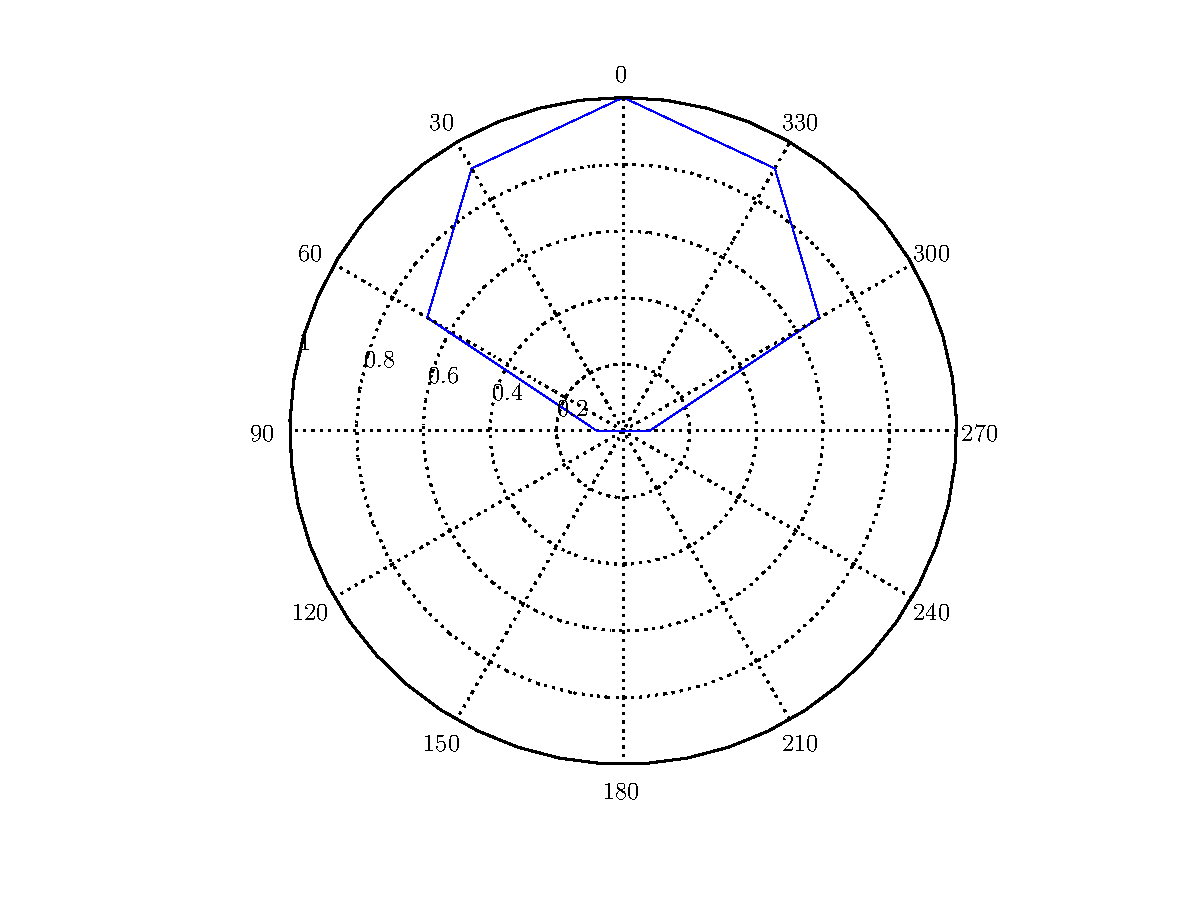
\includegraphics[scale=0.6]{illuminance_angle.pdf}
	\caption{Relationship between the Ring illuminance and the angle to the normal of the Ring surface.}
	\label{fig:illuminance_angle}
\end{figure}
The illuminance decreases as the angle to the normal of the NeoPixel surface increases. Any objects in front of the NeoPixel will receive an illuminance. However, any object behind the NeoPixel will not. This model follows Lambert's Cosine law given by \cref{eq:lambert}. To maximise the illuminance, the object must be on the normal to the surface of the NeoPixel.

\subsubsection{Conclusion of these experiment}
The NeoPixel has the following characteristics:
\begin{itemize}
	\item The illuminance received by an object decreases as the is moved further away from the NeoPixel.
	\item The illuminance received by an object decreases as the is moved at an angle further away from the normal of the NeoPixel.
	\item \textbf{The NeoPixel produces at least 30lx on any object placed in front of the neopixel at a maximum distance of 1m.}
\end{itemize}
\include{body/Discussion}
\chapter{Conclusions and Recommendations}

\section{Review of objectives}
The sub-requirements set in \ref{sub_requirements} and their satisfaction level are shown in \cref{table:conclusion_subrequirements}. The table provides reasons on the satisfaction level given for each requirement.
\begin{table}[h!]
	\centering
	\caption{Sub-requirements implementation satisfaction.}
	\label{table:conclusion_subrequirements}
	\begin{tabular}{p{10em}cp{15em}}
		\hline
		\hline
		\toprule
		\textbf{Sub-requirements} & \textbf{Level of satisfaction} & \textbf{Coments}\\
		\bottomrule
		\toprule
		Onboard touchscreen & High & Good framework design for communication between screen and STM\\
		\midrule
		Smartphone App & Low & Framework is developed but actual application can only connect to bluetooth\\
		\midrule
		User preference & Medium & Framework for storing and loading any parameters have been implemented\\
		\midrule
		Set/edit alarm & High& Good framework allowing alarm configuration\\
		Set/get time and date & High & Good framework allowing time and date parameters to be stored and loaded\\
		\midrule
		Light parameters & Good & Framework allows configuration of the neopixels colour and brightness.\\
		\midrule
		Light pattern & Low & Data sent to neopixels is corrupted by the interrupt generated by other module\\
		\bottomrule
		\hline
		\hline
	\end{tabular}
\end{table}
Each of these sub-requirements is related to the system requirement. \Cref{table:conclusion_requirements} provides the satisfaction lvel of the system requirements. 
\begin{table}[h!]
	\centering
	\caption{Requirements implementation satisfaction.}
	\label{table:conclusion_requirements}
	\begin{tabular}{cc}
		\hline
		\hline
		\toprule
		\textbf{Requirements} & \textbf{Level of satisfaction}\\
		\bottomrule
		\toprule
		Visual & Low \\
		\midrule
		Instruction & High \\
		\midrule
		Alarm & High \\
		\bottomrule
		\hline
		\hline
	\end{tabular}
\end{table}
\subsection{Instruction and user inputs}
The instruction application provided a solid foundation for the implementation of the applications running on each input device. The Nextion touchscreen application provides a nice and easy user interaction with the NPSC. The smartphone application is not fully implemented, the basic interaction provided by this application was connecting the smartphone to the NPSC system. 
\subsection{Alarm}
The alarm application successfully managed the time, date and alarm information of the system. The user has full control of the time, date and the alarm to be set.  
\subsection{Visual}
The visual module was able to control the neopixel at a module level. However, it failed once it was integrated with other modules as they interupted the stream of data sent to the neopixel. For this reason the visual application could not be fully implemented.

\paragraph{Objectives}
\textit{The purpose of this study is to create a device that can be used to regulate the human sleep-wake cycle while being user-friendly and a personalisable digital alarm clock.} \\
The objectives are reviewed in \Cref{table:conclusion_objectives}.
\begin{table}[h!]
	\centering
	\caption{Review of objectives.}
	\label{table:conclusion_objectives}
	\begin{tabular}{p{20em}c}
		\hline
		\hline
		\toprule
		\textbf{Objectives} & \textbf{Comment}\\
		\bottomrule
		\toprule
		The device is capable of producing light of $460\pm10nm$ wavelength at an illuminance of $30lx$ & \checkmark \\
		\midrule
		The device is an alarm clock & \checkmark \\
		\midrule
		The device is user-friendly & \checkmark \\
		\midrule
		The device has more features than its competitors & X \\
		\bottomrule
		\hline
		\hline
	\end{tabular}
\end{table}  

\section{Reflections on the design}
The prototype of the NPSC is proof that the neopixels can be used to create a device capable of affecting the human sleep-wake cycle. However, using a large number of neopixels in an embedded system requires careful use of the microcontroller resources. In this project, the DMA was not used to control the neopixel resulting in the CPU doing all the work from the communication between all modules to the transmission of the neopixels' data. \\
The prototype is subjective to many design changes, therefore, a cost analysis could not be performed. Considering all the module designed for the neopixel, a significant amount of work has been done. All modules have been tested and proven to work creating a solid foundation for future improvements. 

\section{Recommendation for future work}
The following recommendations are firstly made so that all requirements established in the introduction are met, secondly do that the NPSC's design and performance increases over time.\\
The recommendations are the following:
\begin{itemize}
	\item The NPSC's visual module should be dedicated to another microcontroller, preferably an STM32F0 so that the libraries made can be reused. The role of the STM32F0 would solely be to read instruction from the STM32F4 and update the visual output accordingly. This would reduce the workload of the STM32F4 and physically separate the visual module from the other module. 
	\item The neopixel library should make use of the Direct Memory Access (DMA) to reduce the CPU workload.
	\item The experiment performed on the Ring should be done in a completely dark room where the reflection would be minimum to increase the reading accuracy
\end{itemize}
\include{body/Recommendations}
\begin{thebibliography}{5}

%%%%%%%%%%%%%%%%%%%%%%%%%%%%%%%%%%%%%%%%%%%%%%%%%%%%%%%%%%%%%%%%%%%%%%%%%%%%%%%%%%%%
% Circadian Rhythm 
%%%%%%%%%%%%%%%%%%%%%%%%%%%%%%%%%%%%%%%%%%%%%%%%%%%%%%%%%%%%%%%%%%%%%%%%%%%%%%%%%%%%
% GE Lighting, lighting and sleep
\bibitem{ge2014} General Electric Company, ``GE Lighting, lighting and sleep'', December 2014.
% Circadian and Light Effects on Human Sleepiness-Alertness
\bibitem{cir2014} C. Cajochen, S. L. Chellappa and C. Schmidt, ``Circadian and Light Effects on Human Sleepiness-Alertness'', \emph{Sleepiness and Human Impact Assessment}, pp. 9-22, 2014.
% Light, Melatonin and Sleep-Wake Cycle
\bibitem{lig1994} Gregory M. Brown, ``Light, Melatonin and Sleep-Wake Cycle'', \emph{Journal Psychriatry Neurosci}, {\bf vol. 19(5)}, pp. 345-353, Nov 1994.
% Blue light from light-emitting diodes elicits a dose-dependent suppression of melatonin in humans
\bibitem{bl2010} K. E. West, M. R. Jablonski, B. Warfield, K. S. Cecil, M. James, M. A. Ayers, J. Maida, C. Bowen, D. H. Sliney, M. D. Rollag, J. P. Hanifn and G. C. Brainard, ``Blue light from light-emitting diodes elicits a dose-dependent suppression of melatonin in humans'', \emph{Journal Appl Physiol}, {\bf vol. 110}, pp. 619-626, 16 Dec 2010.
% Action Spectrum for Melatonin Regulation in Humans: Evidence for a Novel Circadian Photoreceptor
\bibitem{ac2001} George C. Brainard, John P. Hanifin, Jeffrey M. Greeson, Brenda Byrne, Gena Glickman, Edward Gerner and Mark D. Rollag, ``Action Spectrum for Melatonin Regulation in Humans: Evidence for a Novel Circadian Photoreceptor'', \emph{Journal of Neuroscience}, {\bf vol. 21(16)}, pp. 6405-6412, 15 Au 2001.
% Phototransduction by Retinal Ganglion Cells That Set the Circadian Clock.
\bibitem{ph2002} Berson, D. M., F. A. Dunn, and M. Takao. ``Phototransduction by Retinal Ganglion Cells That Set the Circadian Clock.'' \emph{Science}, {\bf vol. 295}, pp. 1070-073, 2002.
% An action spectrum for melatonin suppression: evidence for a novel non-rod, non-cone photoreceptor system in humans
\bibitem{an2001} Kavita Thapan, Josephine Arendt and Debra J. Skene, ``An action spectrum for melatonin suppression: evidence for a novel non-rod, non-cone photoreceptor system in humans'', \emph{Journal of Physiology}, {\bf vol. 535.1}, pp.261-267, July 2001.
% Dose-response  relationship  for  light  intensity  and  ocular  and electroencephalographic  correlates  of  human  alertness
\bibitem{do2000} Christian  Cajochen*,  Jamie  M.  Zeitzer,  Charles  A.  Czeisler,  Derk-Jan  Dijk, ``Dose-response  relationship  for  light  intensity  and  ocular  and electroencephalographic  correlates  of  human  alertness'', \emph{Behavioural Brain Research }, {\bf vol. 115}, pp.75-83, May 2000.
% Early versus late bedtimes phase shift the human dim light melatonin rhythm despite a fixed morning lights on time
\bibitem{ea2004} Helen J. Burgess and Charmane I. Eastman, ``Early versus late bedtimes phase shift the human dim light melatonin rhythm despite a fixed morning lights on time'', \emph{Neurosci Lett.}, {\bf vol. 356(2)}, pp. 115–118, Feb 2004.
% Home Lighting Before Usual Bedtime Impacts Circadian Timing: A Field Study
\bibitem{ho2014} Helen J. Burgess and Thomas A. Molina, ``Home Lighting Before Usual Bedtime Impacts Circadian Timing: A Field Study'', \emph{Photochem Photobiol.}, {\bf vol. 90(3)}, pp. 723–726, 2014.
% Lighting for Health: LEDs in the New Age of Illumination
\bibitem{ho2014} US Department of Energy, ``Lighting for Health: LEDs in the New Age of Illumination'', \emph{Solid-State Lighting Technology Fact Sheet }, 2014.
% A Working Threshold for Acute Nocturnal Melatonin Suppression from “White”Light Sources used in Architectural Applications
\bibitem{aw2013} Mark S. Rea and Mariana G. Figueiro, ``A Working Threshold for Acute Nocturnal Melatonin Suppression from “White”Light Sources used in Architectural Applications'', \emph{Lighting Research Center, Rensselaer Polytechnic Institute, Troy, New York, USA}, 2013.
% Internal rhythms in humans
\bibitem{in1996} Derk-Jan Dijk, ``Internal rhythms in humans'', \emph{CELL \& DEVELOPMENTAL BIOLOGY}, {\bf vol. 7}, pp. 831-836, 1996.
% Scientific Background Discoveries of Molecular Mechanisms Controlling the Circadian Rhythm
\bibitem{sc2017} ``Scientific Background Discoveries of Molecular Mechanisms Controlling the Circadian Rhythm'', \emph{The Nobel Assembly at Karolinska Institutet}, 2017.
% Is sleep fundamentally different between mammalian species?
\bibitem{is1995} Tobler I., ``Is sleep fundamentally different between mammalian species?'', \emph{Behav Brain Res.}, {\bf vol. 69(1-2)}, pp. 35-41, Jul-Aug 1995.
% GE Sol
\bibitem{gesol} GE sol, [Online], available at: https://www.cbyge.com/products/sol
% Philips
\bibitem{philips} Philips, [Online], available at: https://www.usa.philips.com/c-p/HF3550\_60/discontinued-wake-up-light/overview
% Therapeutics for Circadian Rhythm Sleep Disorders
\bibitem{th2010} Ehren R. Dodson and Phyllis C Zee, ``Therapeutics for Circadian Rhythm Sleep Disorders'', \emph{Sleep Med Clin}, \textbf{vol. 5(4)}, pp. 701-715, Dec 2010.

%%%%%%%%%%%%%%%%%%%%%%%%%%%%%%%%%%%%%%%%%%%%%%%%%%%%%%%%%%%%%%%%%%%%%%%%%%%%%%%%%%%%
% Microcontrollers
%%%%%%%%%%%%%%%%%%%%%%%%%%%%%%%%%%%%%%%%%%%%%%%%%%%%%%%%%%%%%%%%%%%%%%%%%%%%%%%%%%%%
% How Microcontrollers Work
\bibitem{ho2000} Marshall Brain,``How Microcontrollers Work'',\emph{HowStuffWorks.com}[Online] ,available at: http://electronics.howstuffworks.com/microcontroller1.htm, 1 Apr 2000.
% Arduino Due Specifications
\bibitem{arduino} ``Arduino Due Specifications'', \emph{Arduino}, [Online], available at: https://store.arduino.cc/arduino-due
% Intel Edison Specifications
\bibitem{intel} ``Intel Edison Specifications'', \emph{Intel}, [Online], available at: https://cdn-shop.adafruit.com/datasheets/EdisonDatasheet.pdf
% Arduino Due Specifications
\bibitem{raspberry} ``Raspberry Pi Zero Specifications'', \emph{Raspberry Pi}, [Online], available at: https://www.raspberrypi.org/products/raspberry-pi-zero-w/
% Arduino Due Specifications
\bibitem{stm} ``STM32F407VGT6 Specifications'', \emph{STM microelectronics}, [Online], available at: http://www.st.com/en/microcontrollers/stm32f407-417.html?querycriteria=productId=LN11

%%%%%%%%%%%%%%%%%%%%%%%%%%%%%%%%%%%%%%%%%%%%%%%%%%%%%%%%%%%%%%%%%%%%%%%%%%%%%%%%%%%%
% Storage
%%%%%%%%%%%%%%%%%%%%%%%%%%%%%%%%%%%%%%%%%%%%%%%%%%%%%%%%%%%%%%%%%%%%%%%%%%%%%%%%%%%%
% Serial EEPROM Solutions vs. Parallel Solutions
\bibitem{serialvsparallel} Tom Tyson, ``Serial EEPROM Solutions vs. Parallel Solutions'', \emph{Memory Products Division, Microchip}, [Online], available at: http://ecee.colorado.edu/~mcclurel/microchipan551.pdf
% Basic Serial EEPROM Operation
\bibitem{serialoperation} Steve Drehobl, ``Basic Serial EEPROM Operation'', \emph{Memory Products Division, Microchip}, [Online], available at: http://ecee.colorado.edu/~mcclurel/man536.pdf
% Embedded EEPROM Speed Optimization Using System Power Supply Resources
\bibitem{embeddedeeprom} Jean-Michel DagaCaroline, PapaixMarylene CombeEmmanuel, RacapeVincent Sialelli, ``Embedded EEPROM Speed Optimization Using System Power Supply Resources'', \emph{Lecture Notes in Computer Science}, \textbf{vol. 3254}. 

%%%%%%%%%%%%%%%%%%%%%%%%%%%%%%%%%%%%%%%%%%%%%%%%%%%%%%%%%%%%%%%%%%%%%%%%%%%%%%%%%%%%
% Wireless communication
%%%%%%%%%%%%%%%%%%%%%%%%%%%%%%%%%%%%%%%%%%%%%%%%%%%%%%%%%%%%%%%%%%%%%%%%%%%%%%%%%%%%
% Bluetooth in wireless communication
\bibitem{bluetooth} K. V. S. S. S. S. Sairam and N. Gunasekaran and S. R. Redd, ``Bluetooth in wireless communication'', \emph{IEEE Communications Magazine}, \textbf{vol. 40(6)}, pp. 90-96, Jun 2002. 

%%%%%%%%%%%%%%%%%%%%%%%%%%%%%%%%%%%%%%%%%%%%%%%%%%%%%%%%%%%%%%%%%%%%%%%%%%%%%%%%%%%%
% Bluetooth
%%%%%%%%%%%%%%%%%%%%%%%%%%%%%%%%%%%%%%%%%%%%%%%%%%%%%%%%%%%%%%%%%%%%%%%%%%%%%%%%%%%%
% Resistive Touch Screen
\bibitem{resistivetouch} ``Resistive Touch Screen'', \emph{Baanto},[Online], available at: http://baanto.com/resistive-touch-screen-technology
% Capacitive Touch Screen
\bibitem{capacitivetouch} ``Capacitive Touch Screen'', \emph{Baanto},[Online], available at: http://baanto.com/capacitive-touch-screen

%%%%%%%%%%%%%%%%%%%%%%%%%%%%%%%%%%%%%%%%%%%%%%%%%%%%%%%%%%%%%%%%%%%%%%%%%%%%%%%%%%%%
% Communications
%%%%%%%%%%%%%%%%%%%%%%%%%%%%%%%%%%%%%%%%%%%%%%%%%%%%%%%%%%%%%%%%%%%%%%%%%%%%%%%%%%%%
% SPI
\bibitem{spi} ``Serial Peripheral Interface (SPI) '', \emph{Sparkfun},[Online], available at: https://learn.sparkfun.com/tutorials/serial-peripheral-interface-spi
% UART
\bibitem{uart} `` Serial Communication '', \emph{Sparkfun},[Online], available at: https://learn.sparkfun.com/tutorials/serial-communication 
% I2C
\bibitem{i2c} ``I2C'', \emph{Sparkfun},[Online], available at: https://learn.sparkfun.com/tutorials/i2c


%%%%%%%%%%%%%%%%%%%%%%%%%%%%%%%%%%%%%%%%%%%%%%%%%%%%%%%%%%%%%%%%%%%%%%%%%%%%%%%%%%%%
% PCB Design
%%%%%%%%%%%%%%%%%%%%%%%%%%%%%%%%%%%%%%%%%%%%%%%%%%%%%%%%%%%%%%%%%%%%%%%%%%%%%%%%%%%%
% Generic Standard on Printed Board Design
\bibitem{pcb_design} ``Generic Standard on Printed Board Design'', \emph{ASSOCIATION CONNECTING
ELECTRONICS INDUSTRIES},[Online], available at: http://www.sphere.bc.ca/class/downloads/ipc\_2221a-pcb\%20standards.pdf
% Trace Width Website Calculator
\bibitem{pcb_track_width} Advanced Circuits, ``Trace Width Website Calculator'', [Online] available at: http://www.4pcb.com/trace-width-calculator.html


%%%%%%%%%%%%%%%%%%%%%%%%%%%%%%%%%%%%%%%%%%%%%%%%%%%%%%%%%%%%%%%%%%%%%%%%%%%%%%%%%%%%
% Programming
%%%%%%%%%%%%%%%%%%%%%%%%%%%%%%%%%%%%%%%%%%%%%%%%%%%%%%%%%%%%%%%%%%%%%%%%%%%%%%%%%%%%
% Programming in C : A complete intorduction to the C programming language
\bibitem{c_programming} Stephen G. Kochan, ``Programming in C : A complete intorduction to the C programming language, Third Edition''.
% Java: The complete reference, Seventh Edition
\bibitem{java_programming} Herbert Schildt, ``Java: The complete reference, Seventh Edition''.

%%%%%%%%%%%%%%%%%%%%%%%%%%%%%%%%%%%%%%%%%%%%%%%%%%%%%%%%%%%%%%%%%%%%%%%%%%%%%%%%%%%%
% Light
%%%%%%%%%%%%%%%%%%%%%%%%%%%%%%%%%%%%%%%%%%%%%%%%%%%%%%%%%%%%%%%%%%%%%%%%%%%%%%%%%%%%
% Programming in C : A complete intorduction to the C programming language
\bibitem{lighting} Energy Saver, ``Type of lighting'', \emph{U.S Department of Energy}, [Onile] available at: https://energy.gov/energysaver/types-lighting.
% Modern Optical Engineering
\bibitem{optical} Warren J. Smith, ``Modern Optical Engineering: The Design of Optical Systems''


%%%%%%%%%%%%%%%%%%%%%%%%%%%%%%%%%%%%%%%%%%%%%%%%%%%%%%%%%%%%%%%%%%%%%%%%%%%%%%%%%%%%
% Software tool
%%%%%%%%%%%%%%%%%%%%%%%%%%%%%%%%%%%%%%%%%%%%%%%%%%%%%%%%%%%%%%%%%%%%%%%%%%%%%%%%%%%%
% Features
\bibitem{atollic} Atollic TrueSTUDIO, ``Features'', \emph{Atollic TrueSTUDIO}, [Onile] available at: https://atollic.com/truestudio/features/
% Features
\bibitem{nextion} Nextion, ``Features'', \emph{Nextion}, [Onile] available at: https://nextion.itead.cc/
% Features
\bibitem{android} Android, ``Everything you need to build on Android'', \emph{Android}, [Onile] available at: https://developer.android.com/studio/features.html
% paper
\bibitem{ref} authors, ``Paper'', \emph{Journal}, \textbf{vol.}, pp. 
\end{thebibliography}

\appendix
\chapter{Additional Files and Schematics}

%%%%%%%%%%%%%%%%%%%%%%%%%%%%%%%%%%%%%%
% 				RING
\begin{figure}[h!]
	\centering
	\includegraphics[scale=0.55]{ring_sch.pdf}
	\caption{Schematic of the Ring module}
	\label{fig:ring_sch}
\end{figure}

\begin{figure}[h!]
	\centering
	\includegraphics[scale=0.6]{ring_pcb.png}
	\caption{PCB of the Ring module}
	\label{fig:ring_pcb}
\end{figure}
%%%%%%%%%%%%%%%%%%%%%%%%%%%%%%%%%%%%%%
% 				TIME
\begin{figure}[h!]
	\centering
	\includegraphics[scale=0.55]{time_sch.pdf}
	\caption{Schematic of the Time module}
	\label{fig:time_sch}
\end{figure}

\begin{figure}[h!]
	\centering
	\includegraphics[scale=0.55]{time_pcb.png}
	\caption{PCB of the Time module}
	\label{fig:time_pcb}
\end{figure}
%%%%%%%%%%%%%%%%%%%%%%%%%%%%%%%%%%%%%%
% 				WEEKDAY
\begin{figure}[h!]
	\centering
	\includegraphics[scale=0.55]{weekday_sch.pdf}
	\caption{Schematic of the Weekday module}
	\label{fig:weekday_sch}
\end{figure}

\begin{figure}[h!]
	\centering
	\includegraphics[scale=0.4]{weekday_pcb.png}
	\caption{PCB of the Weekday module}
	\label{fig:weekday_pcb}
\end{figure}
%%%%%%%%%%%%%%%%%%%%%%%%%%%%%%%%%%%%%%
% 				DATE
\begin{figure}[h!]
	\centering
	\includegraphics[scale=0.55]{date_sch.pdf}
	\caption{Schematic of the Date module}
	\label{fig:date_sch}
\end{figure}

\begin{figure}[h!]
	\centering
	\includegraphics[scale=0.6]{date_pcb.png}
	\caption{PCB of the Date module}
	\label{fig:date_pcb}
\end{figure}

\chapter{Experiment results}\label{appendix_result}

\begin{table}[h!]
	\centering
	\caption{Current drawn by a one neopixel per colour at different brightness levels. The white colour is obtain by turning the red, green and blue LEDs on at the same brightness.}
	\label{table:current_one_pixel}
	\begin{tabular}{ccccc}
		\hline
		\hline
		\toprule
		\multirow{2}{*}{\textbf{Brightness (\%)}} & \multicolumn{4}{c}{\textbf{Current (mA)}}\\
		& \textbf{Red} & \textbf{Green} & \textbf{Blue} & \textbf{White} \\
		\hline
		\toprule
		\toprule
		0    &    3    &    3    &    3    &    3    \\
		10    &    4    &    4    &    4    &    5    \\
		20    &    5    &    5    &    5    &    9    \\
		30    &    7    &    7    &    6    &    13    \\
		40    &    8    &    8    &    8    &    17    \\
		50    &    10    &    10    &    9    &    22    \\
		60    &    11    &    11    &    11    &    26    \\
		70    &    13    &    12    &    12    &    30    \\
		80    &    14    &    14    &    13    &    34    \\
		90    &    15    &    15    &    15    &    38    \\
		100    &    17    &    17    &    16    &    42    \\
		\bottomrule
		\hline
		\hline
	\end{tabular}
\end{table}
\begin{table}[h!]
	\centering
	\caption{Current drawn by the neopixels in idle mode. The idle mode is defined as the state of the of the neopixel when no light is emitted.}
	\label{table:current_idle}
	\begin{tabular}{cc}
		\hline
		\hline
		\toprule
		\textbf{Number of neopixels} & \textbf{Current (mA)}\\
		\bottomrule
		\toprule
		0    &    89    \\
		10    &    89    \\
		25    &    90    \\
		50    &    92    \\
		90    &    95    \\
		120    &    97    \\
		150    &    99    \\
		180    &    101    \\
		\bottomrule
		\hline
		\hline
	\end{tabular}
\end{table}		
\begin{table}[h!]
	\centering
	\caption{Current drawn by all 180 neopixels on the Ring at different brightness levels.}
	\label{table:current_180_neopixels}
	\begin{tabular}{cccccc}
		\hline
		\hline
		\toprule
		\multirow{2}{*}{\textbf{Brightness (\%)}} & \multicolumn{4}{c}{\textbf{Current (A)}}\\
		& \multicolumn{3}{c}{\textbf{Readings}} & \textbf{Average} & \textbf{Std dev} \\
		\bottomrule
		\toprule
		0	&	0.120	&	0.120	&	0.120	&	0.120	&	0.00	\\
		10	&	0.510	&	0.510	&	0.500	&	0.507	&	0.01	\\
		20	&	1.250	&	1.230	&	1.220	&	1.233	&	0.02	\\
		30	&	2.000	&	1.980	&	1.970	&	1.983	&	0.02	\\
		40	&	2.730	&	2.690	&	2.680	&	2.700	&	0.03	\\
		50	&	3.480	&	3.430	&	3.410	&	3.440	&	0.04	\\
		60	&	4.890	&	4.120	&	4.110	&	4.373	&	0.45	\\
		70	&	4.910	&	4.840	&	4.830	&	4.860	&	0.04	\\
		80	&	5.600	&	5.530	&	5.510	&	5.547	&	0.05	\\
		90	&	6.320	&	6.240	&	6.220	&	6.260	&	0.05	\\
		100	&	7.020	&	6.910	&	6.890	&	6.940	&	0.07	\\
		\bottomrule
		\hline
		\hline
	\end{tabular}
\end{table}				

\begin{table}[h!]
	\centering
	\caption{Temperature rise of the Ring}
	\label{table:temperature_ring}
	\begin{tabular}{cc}
		\hline
		\hline
		\toprule
		\textbf{Current (A)} & \textbf{Temperature ($^oC$)}\\
		\bottomrule
		\toprule
		0.09    &    2.176    \\
		0.49    &    6.417    \\
		1.24    &    11.750    \\
		1.95    &    17.667    \\
		3.38    &    28.083    \\
		4.1        &    29.667    \\
		5.35    &    39.000    \\
		6        &    43.091    \\
		6.55    &    44.750    \\
		\bottomrule
		\hline
		\hline
	\end{tabular}
\end{table}

\begin{table}[h!]
	\centering
	\caption{Ring's blue LED illuminance at full brightness per distance and angular section to the Ring.}
	\label{table:illuminance_blue}
	\begin{tabular}{ccccc}
		\hline
		\hline
		\toprule
		\multirow{2}{*}{\textbf{Distance (cm)}} & \multicolumn{4}{c}{\textbf{Angle (deg)}}\\
		& 0 & 30 & 60 & 90 \\
		\bottomrule
		\toprule
		20    &    6420    &    5950    &    5310    &    1998    \\
		30    &    4910    &    3770    &    3302    &    547        \\
		40    &    2507    &    2354    &    1657    &    149        \\
		50    &    1820    &    1620    &    1219    &    110        \\
		60    &    1375    &    1227    &    892        &    60        \\
		70    &    1012    &    943        &    691        &    55        \\
		80    &    810        &    785        &    547        &    43        \\
		90    &    667        &    607        &    420        &    35        \\
		100    &    557        &    500        &    353        &    30        \\
		\bottomrule
		\hline
		\hline
	\end{tabular}
\end{table}
\begin{table}[h!]
	\centering
	\caption{Relationship between the coefficient of decadence of the Ring illuminance and the distance to the Ring.}
	\label{table:illuminance_distance}
	\begin{tabular}{cccccccc}
		\hline
		\hline
		\toprule
		\multirow{2}{*}{\textbf{Distance (cm)}} & \multicolumn{5}{c}{\textbf{Brightness (\%)}} & \multirow{2}{*}{\textbf{Average}} & \multirow{2}{*}{\textbf{Std dev}}\\
		& 10 & 30 & 50 & 80 & 90 &&\\
		\bottomrule
		\toprule
		20    &    1.00    &    1.00    &    1.00    &    1.00    &    1.00    &    1.00    &    0.00    \\
		30    &    0.68    &    0.63    &    0.65    &    0.65    &    0.59    &    0.64    &    0.03    \\
		40    &    0.44    &    0.40    &    0.44    &    0.41    &    0.36    &    0.41    &    0.03    \\
		50    &    0.31    &    0.29    &    0.31    &    0.28    &    0.27    &    0.29    &    0.02    \\
		60    &    0.23    &    0.20    &    0.23    &    0.22    &    0.20    &    0.22    &    0.01    \\
		70    &    0.18    &    0.15    &    0.18    &    0.17    &    0.15    &    0.17    &    0.01    \\
		80    &    0.14    &    0.13    &    0.14    &    0.13    &    0.12    &    0.13    &    0.01    \\
		90    &    0.12    &    0.10    &    0.11    &    0.13    &    0.10    &    0.11    &    0.01    \\
		100    &    0.10    &    0.08    &    0.09    &    0.09    &    0.08    &    0.09    &    0.01    \\
		\bottomrule
		\hline
		\hline
	\end{tabular}
\end{table}


\begin{table}[h!]
	\centering
	\caption{Relationship between the Ring illuminance and the distance to the Ring.}
	\label{table:illuminance_distance_value}
	\begin{tabular}{cccccccc}
		\hline
		\hline
		\toprule
		\multirow{2}{*}{\textbf{Distance (cm)}} & \multicolumn{5}{c}{\textbf{Brightness (\%)}} & \multirow{2}{*}{\textbf{Average}} & \multirow{2}{*}{\textbf{Std dev}}\\
		& 10 & 30 & 50 & 80 & 90 & 100 &\\
		\bottomrule
		\toprule
20	&	515	&	2870	&	4443	&	7042	&	10000	\\
30	&	351	&	1820	&	2871	&	4573	&	5926	\\
40	&	229	&	1150	&	1947	&	2880	&	3608	\\
50	&	162	&	825	&	1383	&	1982	&	2657	\\
60	&	120	&	587	&	1017	&	1520	&	2042	\\
70	&	92	&	440	&	787	&	1202	&	1500	\\
80	&	74	&	366	&	617	&	925	&	1171	\\
90	&	60	&	291	&	508	&	900	&	970	\\
100	&	52	&	236	&	418	&	610	&	820	\\
		\bottomrule
		\hline
		\hline
	\end{tabular}
\end{table}

\begin{table}[h!]
	\centering
	\caption{Relationship between the Ring illuminance and the angle to the normal of the Ring surface.}
	\label{table:illuminance_angle}
	\begin{tabular}{cccccccc}
		\hline
		\hline
		\toprule
		\multirow{2}{*}{\textbf{Angle (cm)}} & \multicolumn{5}{c}{\textbf{Distance (cm)}} & \multirow{2}{*}{\textbf{Average}} & \multirow{2}{*}{\textbf{Std dev}}\\
		& 20 & 30 & 50 & 80 & 100 &&\\
		\bottomrule
		\toprule
		0    &    1.00    &    1.00    &    1.00    &    1.00    &    1.00    &    1.00    &    0.00    \\
		30    &    0.88    &    0.89    &    0.53    &    0.94    &    0.90    &    0.83    &    0.16    \\
		60    &    0.75    &    0.70    &    0.65    &    0.64    &    0.64    &    0.68    &    0.05    \\
		90    &    0.20    &    0.16    &    0.09    &    0.06    &    0.05    &    0.11    &    0.07    \\
		\bottomrule
		\hline
		\hline
	\end{tabular}
\end{table}

}
\end{document}
